% !TeX program = xelatex
% !TeX options = -shell-escape -synctex=1 -interaction=nonstopmode -file-line-error "%DOC%"
\documentclass[aspectratio=169,11pt]{beamer}

\setbeamertemplate{navigation symbols}{}
\setbeamertemplate{headline}{}
\setbeamertemplate{footline}{}
\setbeamertemplate{frametitle}{}
\setbeamersize{text margin left=0pt, text margin right=0pt}

\usepackage{fontspec}
\setmainfont{Inter}[Ligatures=TeX]
\setsansfont{Inter}[Ligatures=TeX]
\newfontfamily\InterBold{Inter Bold}[Ligatures=TeX]
\newfontfamily\InterSemi{Inter SemiBold}[Ligatures=TeX]

\usepackage{tikz}
\usetikzlibrary{arrows.meta,positioning,calc,shadows.blur}
\usepackage{graphicx}
\usepackage{booktabs}
\usepackage{array}
\usepackage{colortbl}
\usepackage{hhline}
\usepackage{tabularx}

\newcolumntype{L}[1]{>{\raggedright\arraybackslash}m{#1}}
\newcolumntype{C}[1]{>{\centering\arraybackslash}m{#1}}

\definecolor{mvred}{HTML}{F20601}
\definecolor{mvdark}{HTML}{1C1C1E}
\definecolor{mvgray}{HTML}{6E6E73}
\definecolor{cardbg}{HTML}{F5F5F6}
\definecolor{pinkband}{HTML}{FDECEC}
\definecolor{okgreen}{HTML}{1F8A50}
\definecolor{warnorange}{HTML}{C75000}
\definecolor{purpletag}{HTML}{6A35B0}
\definecolor{mvborder}{HTML}{E3D8D8}

\graphicspath{{assets/}{assets/icons/}{../figures/}{figures/}{../figures/complex_eda/}{../figures/complex_eda/markov/}{../figures/complex_eda/model_tag/}{../figures/preprocessing/}{../figures/apps/}{../figures/brand_clf/}{../figures/gliner/}{../figures/general_study/}}

\newcommand{\kicker}[1]{{\color{mvred}\InterBold\fontsize{8}{10}\selectfont\MakeUppercase{#1}}}
\newcommand{\slidetitle}[1]{{\color{mvdark}\InterBold\fontsize{15.5}{18}\selectfont #1}}

\newcommand{\pinknote}[2]{%
  \begin{tikzpicture}
    \node[fill=pinkband, rounded corners=2pt, inner xsep=9pt, inner ysep=5.5pt,
          text width=\dimexpr\textwidth-18pt\relax] {%
      {\color{mvred}\InterBold\fontsize{8}{10}\selectfont #1}\hspace{7pt}{\color{mvdark}\fontsize{8.5}{11}\selectfont #2}};
  \end{tikzpicture}}
\newcommand{\conclusion}[1]{\pinknote{ВЫВОД}{#1}}

\newcommand{\graynote}[2]{%
  \begin{tikzpicture}
    \node[fill=cardbg, rounded corners=2pt, inner xsep=9pt, inner ysep=5.5pt,
          text width=\dimexpr\textwidth-18pt\relax] {%
      {\color{mvdark}\InterBold\fontsize{8}{10}\selectfont #1}\hspace{7pt}{\color{mvdark}\fontsize{8.5}{11}\selectfont #2}};
  \end{tikzpicture}}

\newcommand{\numdot}[1]{%
  \tikz[baseline=-0.6ex]{\node[circle, fill=mvred, text=white, inner sep=1pt, minimum size=12pt, font=\InterBold\fontsize{7}{8}\selectfont]{#1};}}

\newcommand{\cornerlogo}{%
  \begin{tikzpicture}[remember picture, overlay]
    \node[anchor=north east, xshift=-0.5cm, yshift=-0.38cm] at (current page.north east)
      {
\includegraphics[height=0.85cm]{m_letter.png}};
  \end{tikzpicture}}

\newcommand{\slidehead}[2]{%
  \cornerlogo
  \vspace{0.38cm}\par
  \hspace{0.85cm}\begin{minipage}{\dimexpr\paperwidth-1.7cm\relax}
  \kicker{#1}\par\vspace{3pt}
  \slidetitle{#2}\par\vspace{7pt}}
\newcommand{\slidefoot}{\end{minipage}}

\newcommand{\bodytext}{\fontsize{8.5}{11.5}\selectfont}
\newcommand{\smalltext}{\fontsize{7.5}{10}\selectfont}

\definecolor{tblline}{HTML}{DDDDDD}
\arrayrulecolor{tblline}
\newcommand{\ttext}{\fontsize{7}{9}\selectfont}
\newcommand{\thead}[1]{\cellcolor{mvdark}{\color{white}\InterSemi\ttext #1}}
\newcommand{\theadl}[1]{\cellcolor{mvdark}{\color{white}\InterSemi\ttext #1}}
\newcommand{\tacc}[1]{\cellcolor{mvred}{\color{white}\InterSemi\ttext #1}}
\newcommand{\tcellc}[1]{{\ttext\color{mvdark}#1}}
\newcommand{\tcelll}[1]{{\ttext\color{mvdark}#1}}
\newcommand{\hnum}[1]{{\InterBold\color{mvdark}#1}}
\newcommand{\hb}[1]{{\InterSemi\color{mvdark}#1}}
\newcommand{\tnote}[1]{{\color{mvred}\itshape\fontsize{7}{9}\selectfont #1}}
\newcommand{\dqhead}[1]{{\InterSemi\color{mvgray}#1}}
\newcommand{\dqorig}[1]{{\color{mvgray}#1}}

\newcommand{\appshot}[2]{%
\begin{tikzpicture}
  \node[rounded corners=3pt, inner sep=1.5pt, fill=white, draw=mvborder, line width=0.5pt,
        blur shadow={shadow blur steps=8, shadow xshift=0pt, shadow yshift=-1.2pt,
                     shadow blur radius=2.4pt, shadow opacity=22}]
    {\includegraphics[#1]{#2}};
\end{tikzpicture}}

\newcommand{\wtag}[2]{\tikz[baseline=-0.55ex]{\node[rounded corners=2pt, fill=#1, inner xsep=4pt, inner ysep=2.2pt, font=\InterSemi\fontsize{7.8}{9}\selectfont, text=white]{#2};}}
\newcommand{\wplain}[1]{\tikz[baseline=-0.55ex]{\node[rounded corners=2pt, fill=cardbg, inner xsep=4pt, inner ysep=2.2pt, font=\fontsize{7.8}{9}\selectfont, text=mvdark]{#1};}}
\newcommand{\biotag}[2]{\tikz[baseline=-0.55ex]{\node[rounded corners=1.5pt, fill=#1, inner xsep=2.5pt, inner ysep=1pt, font=\fontsize{6.5}{7.5}\selectfont\color{white}]{#2};}}

\newcommand{\chevron}{%
  \raisebox{-0.15ex}{\begin{tikzpicture}
    \draw[mvred, line width=1.3pt, line cap=round, line join=round]
      (0,0.13) -- (0.065,0.065) -- (0,0);
  \end{tikzpicture}}}
\newcommand{\pipestep}[3]{%
  \begin{tikzpicture}[baseline=(b.center)]
    \node[fill=#1, rounded corners=3pt, minimum height=0.92cm, text width=1.72cm,
          align=center, inner sep=2.5pt, font=\InterSemi\fontsize{6.6}{8}\selectfont, text=#2] (b) {#3};
  \end{tikzpicture}}
\newcommand{\pipestepn}[3]{%
  \begin{tikzpicture}[baseline=(b.center)]
    \node[fill=#1, rounded corners=3pt, minimum height=0.88cm, text width=1.48cm,
          align=center, inner sep=2pt, font=\InterSemi\fontsize{5.8}{7}\selectfont, text=#2] (b) {#3};
  \end{tikzpicture}}
\newcommand{\iconcardsm}[3]{%
  \begin{tikzpicture}
    \node[fill=cardbg, rounded corners=4pt, inner sep=5pt, text width=2.75cm, align=center,
          minimum height=1.95cm, anchor=north] (c) {%
      {\InterSemi\fontsize{7.6}{9.4}\selectfont\color{mvdark}#1}\par\vspace{2pt}
      {\fontsize{6.3}{8}\selectfont\color{mvgray}#2#3}};
  \end{tikzpicture}}
\newcommand{\pipestepq}[3]{%
  \begin{tikzpicture}[baseline=(b.center)]
    \node[fill=#1, rounded corners=3pt, minimum height=0.78cm, text width=1.4cm,
          align=center, inner sep=2pt, font=\InterSemi\fontsize{6.2}{7.6}\selectfont, text=#2] (b) {#3};
  \end{tikzpicture}}
% day3 cards with icons
\newcommand{\iconcard}[3]{%
  \begin{tikzpicture}
    \node[fill=cardbg, rounded corners=4pt, inner sep=6pt, text width=2.7cm, align=center,
          minimum height=2.05cm, anchor=north] (c) {%
      \includegraphics[height=0.68cm]{#1}\par\vspace{3pt}
      {\InterSemi\fontsize{7.5}{9.5}\selectfont\color{mvdark}#2}\par\vspace{2pt}
      {\fontsize{6.4}{8}\selectfont\color{mvgray}#3}};
  \end{tikzpicture}}
% day4 text cards (no icon file)
\newcommand{\iconcardtxt}[3]{%
  \begin{tikzpicture}
    \node[fill=cardbg, rounded corners=4pt, inner sep=6pt, text width=3.05cm, align=center,
          minimum height=2.05cm, anchor=north] (c) {%
      {\InterSemi\fontsize{8}{10}\selectfont\color{mvdark}#1}\par\vspace{3pt}
      {\fontsize{6.6}{8.4}\selectfont\color{mvgray}#2#3}};
  \end{tikzpicture}}

\newcommand{\daydivider}[3]{%
\begin{frame}[plain]
\begin{tikzpicture}[remember picture, overlay]
  \fill[mvdark] (current page.south west) rectangle (current page.north east);
  \node[anchor=west, align=left] at ([xshift=0.9cm, yshift=0.55cm]current page.west)
    {\color{mvred}\InterBold\fontsize{12}{14}\selectfont #1};
  \node[anchor=west, align=left, text width=0.88\paperwidth] at ([xshift=0.9cm, yshift=-0.35cm]current page.west)
    {\color{white}\InterBold\fontsize{22}{26}\selectfont #2};
  \node[anchor=west, align=left, text width=0.85\paperwidth] at ([xshift=0.9cm, yshift=-1.55cm]current page.west)
    {\color{white!80}\fontsize{11}{14}\selectfont #3};
\end{tikzpicture}
\end{frame}}

\setlength{\parskip}{0pt}

\begin{document}

% ============================================================
% ТИТУЛ
% ============================================================
\begin{frame}[plain]
\begin{tikzpicture}[remember picture, overlay]
  \fill[mvred] (current page.south west) rectangle (current page.north east);
  \node[anchor=east, inner sep=0pt] at ([xshift=0.32\paperwidth]current page.east)
    {
\includegraphics[height=1.06\paperheight]{kurs1_image1.png}};
  \node[anchor=west, align=left] at ([xshift=0.9cm, yshift=2.15cm]current page.west)
    {\color{white}\InterBold\fontsize{10}{12}\selectfont БУТКЕМП М.ВИДЕО · NLP / SEARCH · ИТОГИ};
  \node[anchor=west, align=left] at ([xshift=0.88cm, yshift=0.95cm]current page.west)
    {\color{white}\InterBold\fontsize{26}{30}\selectfont Умный поиск:};
  \node[anchor=west, align=left] at ([xshift=0.88cm, yshift=0.05cm]current page.west)
    {\color{white}\InterBold\fontsize{26}{30}\selectfont от данных до каскада};
  \node[anchor=west, align=left, text width=0.52\paperwidth] at ([xshift=0.9cm, yshift=-1.85cm]current page.west)
    {\color{white}\fontsize{11}{14.5}\selectfont Как мы научились понимать поисковый запрос: разобрали данные, собрали MVP, починили опечатки, проверили модели и выложили сервис с честными метриками.};
  \node[anchor=south west] at ([xshift=0.9cm, yshift=0.5cm]current page.south west)
    {\color{white}\fontsize{9}{11}\selectfont Итоговая презентация · Дни 02--05};
\end{tikzpicture}
\end{frame}

\daydivider{ДЕНЬ 02}{Качество данных и постановка}{Дыры в датасете, транслит, раскладка, дубли брендов — и почему задача не «обычный NER».}

\begin{frame}[t]
\slidehead{качество данных · обзор}{Что нашли, когда прочитали данные руками}
\begin{columns}[T]
\column{0.5\textwidth}
\vspace{2pt}\centering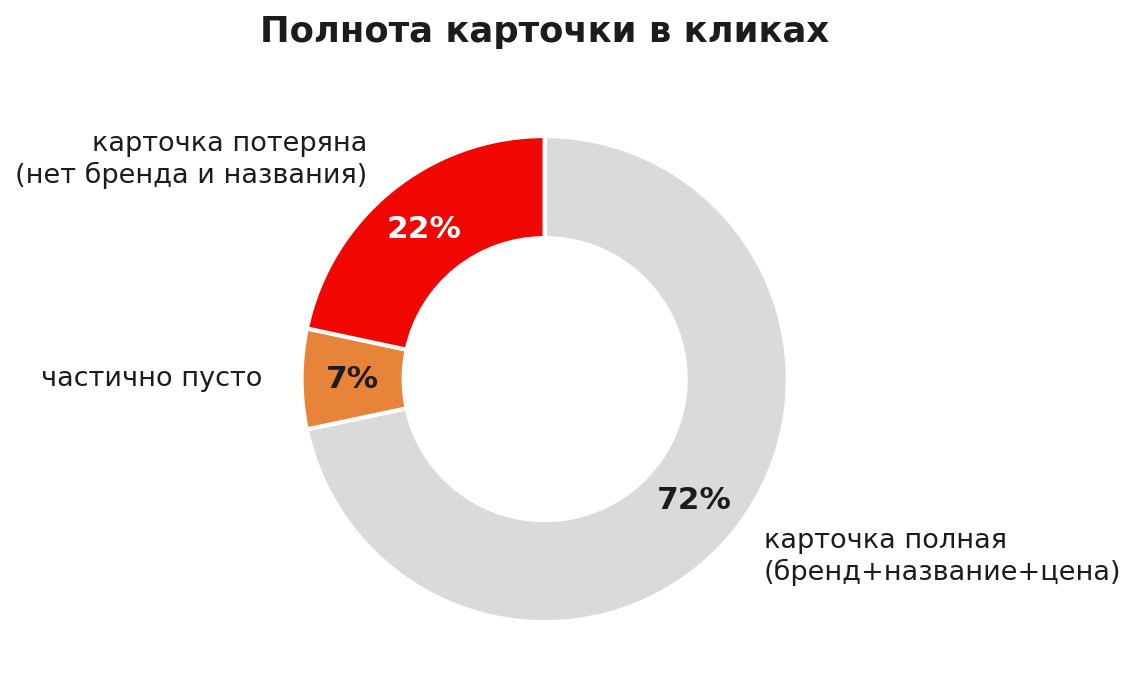
\includegraphics[width=0.90\textwidth]{eda_dq_completeness.png}
\column{0.47\textwidth}
\conclusion{Датасет собирал человек — в нём есть системные дыры и ошибки. Их надо чистить до обучения, иначе модель учится на мусоре.}
\vspace{6pt}\par
{\smalltext
\numdot{1}\ Только \textbf{72\%} кликов имеют полную карточку (бренд + название + цена).\par\vspace{4pt}
\numdot{2}\ У \textbf{22\%} карточка вообще не подтянулась — пусты и бренд, и название (join не срослось при сборке).\par\vspace{4pt}
\numdot{3}\ Формальных \texttt{NaN} нет — дыры спрятаны в пустых строках \texttt{""}, их легко не заметить.}
\end{columns}
\slidefoot
\end{frame}

\begin{frame}[t]
\slidehead{качество данных · перепутанные колонки}{Артикул уехал в поле бренда}
\conclusion{В 66 строках \textbf{бренд — это просто число}. В 98,5\% случаев это артикул из середины названия, попавший не в ту колонку.}
\vspace{8pt}\par
{\renewcommand{\arraystretch}{1.4}\setlength{\tabcolsep}{6pt}
\begin{tabular}{|L{7.4cm}|C{2.3cm}|C{2.5cm}|}
\hline
\theadl{Название товара (sku\_name)} & \thead{Поле «бренд»} & \thead{Реальность}\\
\hline
\tcelll{Вентилятор напольный \hb{27942} GL 8112} & \tcellc{\hb{27942}} & \tacc{артикул}\\
\hline
\tcelll{Камера видеонаблюдения \hb{360} V380 Pro APP} & \tcellc{\hb{360}} & \tacc{артикул}\\
\hline
\tcelll{Туфли женские \hb{0} Туфли} & \tcellc{\hb{0}} & \tacc{заглушка}\\
\hline
\tcelll{Бритва \hb{4088} Extra Smooth Embrace} & \tcellc{\hb{4088}} & \tacc{артикул}\\
\hline
\end{tabular}}
\vspace{6pt}\par
{\smalltext\color{mvgray} Правило для нас: числовой \texttt{sku\_brand\_name} — не бренд, а шум. Реальный бренд ищем в тексте названия либо считаем, что его нет.}
\slidefoot
\end{frame}

\begin{frame}[t]
\slidehead{качество данных · транслит}{Транслит, смесь языков и омоглифы}
\begin{columns}[T]
\column{0.52\textwidth}
\vspace{2pt}\centering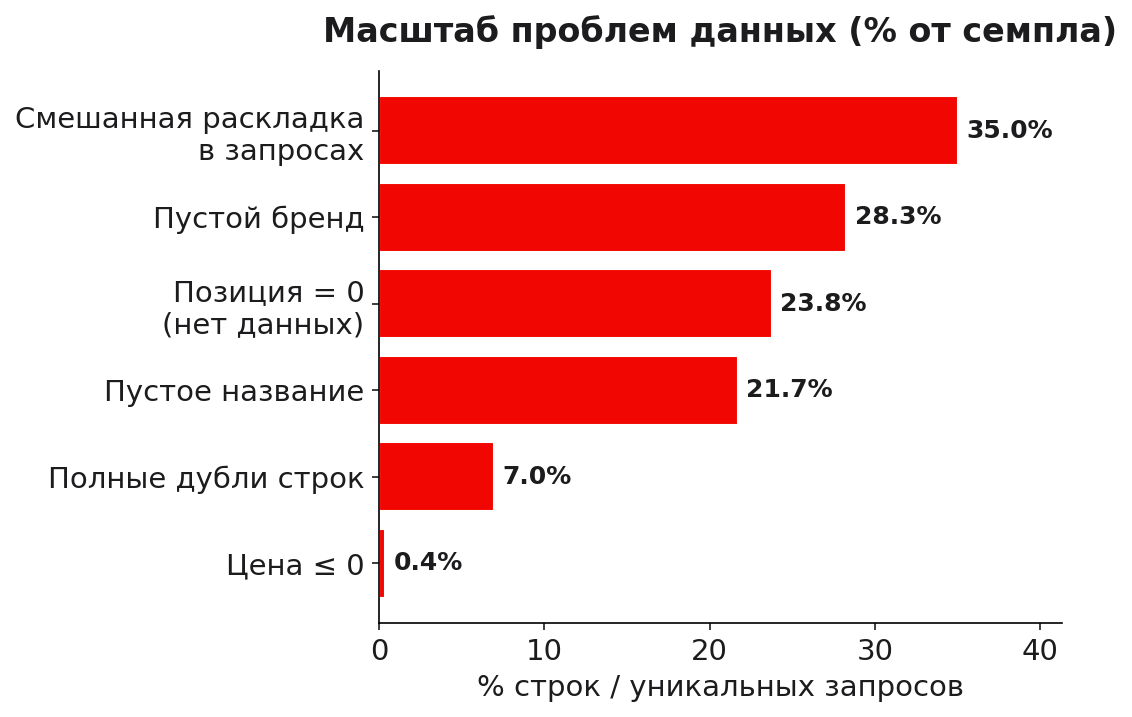
\includegraphics[width=0.98\textwidth]{eda_dq_issues.png}
\column{0.45\textwidth}
\conclusion{\textbf{35\%} уникальных запросов — смесь кириллицы и латиницы. Модель обязана быть устойчива к раскладке.}
\vspace{5pt}\par
{\renewcommand{\arraystretch}{1.05}\setlength{\tabcolsep}{5pt}
\begin{tabular}{|L{2.3cm}|L{3.9cm}|}
\hline
\theadl{Тип} & \theadl{Пример из данных}\\
\hline
\tcelll{\hb{Смесь}} & \tcelll{«iPhone 17 про Макс», «bosh лодильник»}\\
\hline
\tcelll{\hb{Транслит}} & \tcelll{«noutbuk», «televizor», «Stiralnay»}\\
\hline
\tcelll{\hb{Омоглиф}} & \tcelll{«Ресантa» (а — кир.), «Фаzа»}\\
\hline
\tcelll{\hb{Раскладка}} & \tcelll{«dfhjxyfz» {\color{mvred}$\to$} «варочная»}\\
\hline
\end{tabular}}
\end{columns}
\slidefoot
\end{frame}

\begin{frame}[t]
\slidehead{качество данных · забытая раскладка}{Печатали по-русски в EN-раскладке}
\conclusion{Нашли \textbf{80+} запросов вида «dfhjxyfz gfytkm» — это «варочная панель», набранное в латинской раскладке. Поиск обязан их авто-исправлять.}
\vspace{-2pt}\par
{\fontsize{6.0}{7.8}\selectfont\setlength{\tabcolsep}{5pt}\renewcommand{\arraystretch}{1.15}
\begin{columns}[T]
\column{0.49\textwidth}
\begin{tabular}{@{}L{3.0cm}@{\ }L{3.4cm}@{}}
\dqhead{Ввели (EN)} & \dqhead{Хотели найти}\\[2pt]
\dqorig{lkz djkjc aty gkjqrf gkjqrf} & {для волос фен плойка плойка} \\
\dqorig{pfhzlyst ecnhjqcndf lkz frrevekjnjhjd fdnj} & {зарядные устройства для аккумулоторов авто} \\
\dqorig{dfhjxyfz gfytkm ,tkjt cntrkh} & {варочная панель белое стеклр} \\
\dqorig{dbltjrfvthf lkz gjvtotybz} & {видеокамера для помещения} \\
\dqorig{dcnhfbdftvfz cnbhfkmyfz vfibyf} & {встраиваемая стиральная машина} \\
\dqorig{le[jdjq irfa 'ktrnhbxtcrbq} & {духовой шкаф электрический} \\
\dqorig{pfhzlyjt ecnhjqcndj czjvb} & {зарядное устройство сяоми} \\
\dqorig{rf,tkm lkz rkfdbfnehs} & {кабель для клавиатуры} \\
\dqorig{gsktcjc dthnbrfkmysq ghjdjlyjq} & {пылесос вертикальный проводной} \\
\dqorig{nhbvvth lkz yjcf} & {триммер для носа} \\
\dqorig{'ktrnhbxtcrfz gkbnf akfvf} & {электрическая плита флама} \\
\dqorig{,tujdfz ljhj;rf} & {беговая дорожка} \\
\dqorig{,tcghjdjlyjq gsktcjc} & {беспроводной пылесос} \\
\end{tabular}
\column{0.49\textwidth}
\begin{tabular}{@{}L{3.0cm}@{\ }L{3.4cm}@{}}
\dqhead{Ввели (EN)} & \dqhead{Хотели найти}\\[2pt]
\dqorig{dtynbkznjh yfcnjkmysq} & {вентилятор настольный} \\
\dqorig{dthnbrfkmysq gsktcjc} & {вертикальный пылесос} \\
\dqorig{dcnhfbbdftvsq [jkjlbkmybr} & {встраииваемый холодильник} \\
\dqorig{dcnhjtyyfz gjceljvjqrf} & {встроенная посудомойка} \\
\dqorig{dcnhjtyysq [jkjlbkmybr} & {встроенный холодильник} \\
\dqorig{ufpjdfz gkbnf} & {газовая плита} \\
\dqorig{ufqrjdthn htldthu} & {гайковерт редверг} \\
\dqorig{ukflbkmyfz ljcrf} & {гладильная доска} \\
\dqorig{lhtkm ,eh} & {дрель бур} \\
\dqorig{pfdfhjxysq xfqybr} & {заварочный чайник} \\
\dqorig{pfhzlyjt ecnhjqcndj} & {зарядное устройство} \\
\dqorig{buhjdjt rhtckj} & {игровое кресло} \\
\dqorig{buhjdjq hekm} & {игровой руль} \\
\dqorig{rkfdbfnehf ,tkfz} & {клавиатура белая} \\
\end{tabular}
\end{columns}}
\vspace{3pt}\par
{\smalltext\color{mvgray} Детект дешёвый — одна таблица QWERTY$\leftrightarrow$ЙЦУКЕН, ловится в «голове» каскада рядом с regex.}
\slidefoot
\end{frame}

\begin{frame}[t]
\slidehead{качество данных · дубли и меры}{Дубли брендов и что мы с этим делаем}
\begin{columns}[T]
\column{0.5\textwidth}
{\InterSemi\fontsize{8.5}{10.5}\selectfont Один бренд — много написаний}\par\vspace{5pt}
{\renewcommand{\arraystretch}{1.3}\setlength{\tabcolsep}{5pt}
\begin{tabular}{|L{3.0cm}|L{3.4cm}|}
\hline
\theadl{Проблема} & \theadl{Пример}\\
\hline
\tcelll{Регистр} & \tcelll{APPLE / Apple, honor / HONOR}\\
\hline
\tcelll{Перевод} & \tcelll{Stinol / Стинол, KION / КИОН}\\
\hline
\tcelll{Дубли строк} & \tcelll{один клик записан по 2--3 раза}\\
\hline
\end{tabular}}
\vspace{5pt}\par
{\smalltext\color{mvgray} 205 групп брендов различаются лишь регистром/пробелами, $\sim$209 групп — кандидаты на омоглифы.}
\column{0.48\textwidth}
{\InterSemi\fontsize{8.5}{10.5}\selectfont Меры (слой нормализации)}\par\vspace{6pt}
{\smalltext
\numdot{1}\ Приводим бренды к канону: регистр, транслит, схлопывание дублей (\textbf{Стинол}=\textbf{Stinol}).\par\vspace{5pt}
\numdot{2}\ Фильтруем мусор до обучения: пустые карточки и цена $\le$0 — вон или в отдельную метку.\par\vspace{5pt}
\numdot{3}\ Позиция \texttt{= 0} — это «нет данных», не топ выдачи; не используем как сигнал.\par\vspace{5pt}
\numdot{4}\ Это прямой аргумент за \textbf{H5}: одним regex единообразие не навести.}
\end{columns}
\slidefoot
\end{frame}

\begin{frame}[t]
\slidehead{постановка · переосмысление}{Задача — не «обычный NER»}
\conclusion{Главная цель — максимизировать покрытие edge-cases, а не выбить красивый F1 на простых запросах.}
\vspace{12pt}\par
\begin{columns}[T]
\column{0.48\textwidth}
{\InterSemi\fontsize{8.5}{10.5}\selectfont Почему так}\par\vspace{6pt}
{\smalltext
\numdot{1}\ Голова запросов решается словарём за день — это не подвиг.\par\vspace{5pt}
\numdot{2}\ Конверсию теряют хвосты: опечатки, редкие бренды, склейки, смесь языков.\par\vspace{5pt}
\numdot{3}\ Ценность решения = сколько хвоста мы покрываем при SLA $<$ 100 мс.}
\column{0.48\textwidth}
\begin{tikzpicture}
\node[fill=cardbg, rounded corners=3pt, inner sep=7pt, text width=\dimexpr\textwidth-14pt\relax]{
{\InterSemi\fontsize{8.5}{10.5}\selectfont Работаем в вероятностном пространстве}\par\vspace{5pt}
{\smalltext\color{mvgray} Каждый слой отдаёт не только ответ, но и уверенность. Если уверенность низкая — запрос уходит на слой тяжелее. Так простое остаётся быстрым, а сложное — решаемым.}
};
\end{tikzpicture}
\end{columns}
\slidefoot
\end{frame}

\begin{frame}[t]
\slidehead{архитектура · слои}{Три слоя: голова, середина, хвост}
\begin{center}
\begin{tikzpicture}[
  lay/.style={rounded corners=3pt, inner sep=7pt, text width=3.3cm, align=left, minimum height=2.4cm},
  arr/.style={-{Stealth[length=2.6mm]}, line width=1pt, mvgray}
]
  \node[lay, fill=cardbg] (l1) at (0,0)
    {{\color{mvred}\InterBold\small ГОЛОВА}\par\vspace{3pt}
     {\InterSemi\footnotesize regex + правила + словари}\par\vspace{4pt}
     {\fontsize{8}{10.5}\selectfont\color{mvgray}частые и простые запросы; мгновенно, прозрачно, дёшево}};
  \node[lay, fill=cardbg] (l2) at (5.55,0)
    {{\color{mvred}\InterBold\small СЕРЕДИНА}\par\vspace{3pt}
     {\InterSemi\footnotesize CRF и аналоги}\par\vspace{4pt}
     {\fontsize{8}{10.5}\selectfont\color{mvgray}token-level: BIO и другие схемы, либо переход к span-level разметке}};
  \node[lay, fill=mvdark] (l3) at (11.1,0)
    {{\color{mvred}\InterBold\small ХВОСТ}\par\vspace{3pt}
     {\color{white}\InterSemi\footnotesize трансформеры + LLM \textbf{ИЛИ} RNN}\par\vspace{4pt}
     {\fontsize{8}{10.5}\selectfont\color{white!75!mvdark}edge-cases, которые не решаются правилами и обычной NER-моделью}};
  \draw[arr] (l1.east) -- node[above=2.5pt, font=\fontsize{6.5}{7.5}\selectfont\color{mvgray}]{низкая увер.} (l2.west);
  \draw[arr] (l2.east) -- node[above=2.5pt, font=\fontsize{6.5}{7.5}\selectfont\color{mvgray}]{низкая увер.} (l3.west);
\end{tikzpicture}
\end{center}
\vspace{8pt}\par
\conclusion{Каскад по уверенности: 90\% трафика решают дешёвые слои, тяжёлые модели работают только там, где реально нужны.}
\slidefoot
\end{frame}

\begin{frame}[t]
\slidehead{честные метрики · дымовой тест}{CRF на слабой BIO-разметке: ранний smoke-тест}
\conclusion{Метрики на серебряных метках оптимистичны — это ориентир, а не финальная оценка. Сейчас есть gold-holdout и журнал метрик; полный gold доразмечаем приложением.}
\vspace{8pt}\par
\begin{columns}[T]
\column{0.42\textwidth}
{\InterSemi\fontsize{8.5}{10.5}\selectfont Быстрый тест на выборке}\par\vspace{5pt}
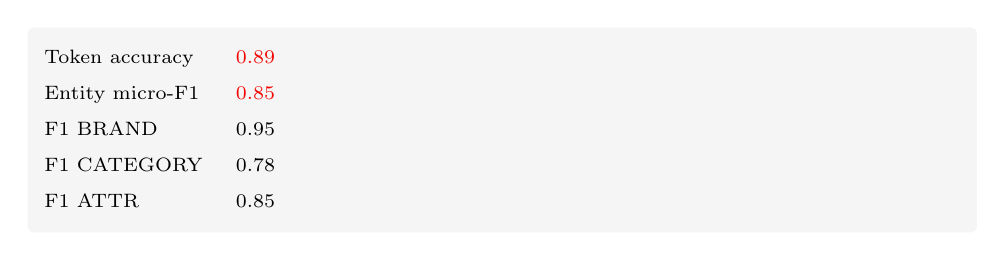
\begin{tikzpicture}[
  st/.style={rounded corners=2pt, fill=cardbg, inner sep=6pt, text width=\dimexpr\textwidth-14pt\relax, font=\smalltext}
]
\node[st]{
\begin{tabular}{@{}ll@{}}
Token accuracy & \InterBold\color{mvred}0.89\\[3pt]
Entity micro-F1 & \InterBold\color{mvred}0.85\\[3pt]
F1 BRAND & \InterBold 0.95\\[3pt]
F1 CATEGORY & \InterBold 0.78\\[3pt]
F1 ATTR & \InterBold 0.85\\
\end{tabular}};
\end{tikzpicture}
\column{0.54\textwidth}
{\InterSemi\fontsize{8.5}{10.5}\selectfont Что это значит}\par\vspace{5pt}
{\smalltext
\numdot{1}\ BRAND учится легко (0.95) — словарь почти решает задачу в голове каскада.\par\vspace{4pt}
\numdot{2}\ CATEGORY слабее (0.78) — формулировки разнообразнее, тут нужен либо трансформер, либо больше слабо-размеченных данных.\par\vspace{4pt}
\numdot{3}\ Итог: CRF — рабочая середина каскада, но категорию и хвост дотягиваем следующим слоем.}
\end{columns}
\slidefoot
\end{frame}

\begin{frame}[t]
\slidehead{eda · проверка гипотез}{Гипотезы: что подтвердилось}
{\renewcommand{\arraystretch}{1.28}\setlength{\tabcolsep}{6pt}
\begin{tabular}{|L{6.4cm}|C{2.0cm}|C{4.0cm}|}
\hline
\theadl{Гипотеза} & \thead{Статус} & \theadl{Комментарий}\\
\hline
\tcelll{\hnum{H1.} Запросы — короткие категорийные интенты} & \tacc{Да} & \tcellc{топы — чистые категории}\\
\hline
\tcelll{\hnum{H2.} Клики концентрируются в топе выдачи} & \tacc{Да} & \tcellc{медиана позиции = 4}\\
\hline
\tcelll{\hnum{H3.} Бренд в запросе $\Rightarrow$ клик того же бренда} & \tcellc{В основном} & \tcellc{heatmap диагональна}\\
\hline
\tcelll{\hnum{H4.} Цена сильно влияет на позицию клика} & \tcellc{Нет} & \tcellc{hexbin: связь слабая}\\
\hline
\tcelll{\hnum{H5.} Атрибуты пишут единообразно} & \tcellc{Нет} & \tcellc{«16гб», «16 gb», «16 ГБ»}\\
\hline
\tcelll{\hnum{H6.} Бренд обычно написан в запросе} & \tcellc{Нет} & \tcellc{только 27\% — нужен классификатор}\\
\hline
\end{tabular}}
\vspace{5pt}\par
\tnote{Красное = подтверждено данными. H5 — атрибуты пишут как попало: одним regex не закрыть, нужен отдельный классификатор типов.}
\slidefoot
\end{frame}

\begin{frame}[t]
\slidehead{обновление · разметка}{Что тогда уже работало: лемматизация}
\conclusion{К тому моменту подключили лемматизацию (Natasha) — словарь начал ловить любые словоформы: «холодильникАМИ», «краснУЮ», «стиральнУЮ машинУ».}
\vspace{6pt}\par
\begin{columns}[T]
\column{0.5\textwidth}
{\InterSemi\fontsize{8.5}{10.5}\selectfont Что уже умели}\par\vspace{5pt}
{\smalltext
\numdot{1}\ Лемматизация: «холодильникАМИ» становится «холодильник» — категория находится, даже если слово склонено. Это прямо чинило слабый CATEGORY-recall.\par\vspace{4pt}
\numdot{2}\ Атрибутов regex стало \textbf{18} вместо 7: память, размер, мощность, ток, вес, объём, частота, гарантия и др.\par\vspace{4pt}
\numdot{3}\ Расклейка склеек: «16гб» превращается в «16 гб», спаны атрибутов стали точными.}
\column{0.48\textwidth}
\begin{tikzpicture}
\node[fill=cardbg, rounded corners=3pt, inner sep=8pt, text width=\dimexpr\textwidth-16pt\relax]{
{\InterSemi\fontsize{8.5}{10.5}\selectfont Пример разбора}\par\vspace{5pt}
{\fontsize{8}{11}\selectfont\color{mvdark}
запрос: «стиральную машину haier белую»\par\vspace{4pt}
бренд: \textbf{Haier}\par
категория: \textbf{стиральная машина}\par
атрибуты: цвет = \textbf{белую}}
};
\end{tikzpicture}
\end{columns}
\slidefoot
\end{frame}

\begin{frame}[t]
\slidehead{архитектура · латентность и SLA}{Как держим SLA $<$ 100 мс с лемматизацией}
\conclusion{Нейромодель Natasha грузится 1 раз при старте (\textasciitilde{}1 с), а сам разбор запроса — \textbf{$<$1 мс}. Онлайн-лемматизация в SLA укладывается, но голову трафика кэшируем.}
\vspace{8pt}\par
\begin{columns}[T]
\column{0.46\textwidth}
{\InterSemi\fontsize{8.5}{10.5}\selectfont Замеры (наш семпл)}\par\vspace{5pt}
\begin{tikzpicture}[st/.style={rounded corners=2pt, fill=cardbg, inner sep=6pt, text width=\dimexpr\textwidth-14pt\relax, font=\smalltext}]
\node[st]{
\begin{tabular}{@{}ll@{}}
Загрузка модели (старт) & \InterBold\color{warnorange}\textasciitilde{}965 мс\\[3pt]
Лемматизация 1 запроса & \InterBold\color{okgreen}\textasciitilde{}0.6 мс\\[3pt]
Токенизация & \InterBold\color{okgreen}0.007 мс\\[3pt]
Бюджет SLA & \InterBold 100 мс\\
\end{tabular}};
\end{tikzpicture}
\par\vspace{5pt}
{\smalltext\color{mvgray} Модель загружается один раз при инициализации сервиса, а не на каждый запрос — поэтому старт не влияет на латентность ответов.}
\column{0.5\textwidth}
{\InterSemi\fontsize{8.5}{10.5}\selectfont Что кэшируем / планируем}\par\vspace{6pt}
{\smalltext
\numdot{1}\ \textbf{Леммы словарей} — считаем один раз офлайн при сборке лейблера, а не на каждый запрос.\par\vspace{5pt}
\numdot{2}\ \textbf{Результат по запросу} (LRU-кэш): голова трафика — это одни и те же запросы; 90\% кликов дают лишь 60\% уникальных строк.\par\vspace{5pt}
\numdot{3}\ \textbf{Леммы токенов} — кэш «словоформа $\to$ лемма»: слова повторяются, второй раз не считаем.\par\vspace{4pt}
\numdot{4}\ Фолбэк: без Natasha «голова» каскада (regex + словарь) работает — деградируем мягко.}
\end{columns}
\slidefoot
\end{frame}


\daydivider{ДЕНЬ 03}{MVP: предобработка, MODEL, каскад}{Единый слой очистки, тег MODEL, brand\_clf, приложения поиска и разметки.}

\begin{frame}[t]
\slidehead{предобработка · пайплайн}{Единый слой очистки запроса}
\begin{columns}[T]
\column{0.52\textwidth}
{\InterSemi\fontsize{8.5}{10.5}\selectfont Шесть шагов очистки}\par\vspace{5pt}
{\renewcommand{\arraystretch}{1.22}\setlength{\tabcolsep}{5pt}
\begin{tabular}{|L{2.4cm}|L{4.2cm}|}
\hline
\theadl{Шаг} & \theadl{Что делает}\\
\hline
\tcelll{\hb{Базовая чистка}} & \tcelll{убирает мусорные пробелы, ё $\to$ е}\\
\hline
\tcelll{\hb{Расклейка}} & \tcelll{«128гб» $\to$ «128 гб»}\\
\hline
\tcelll{\hb{Сепараторы}} & \tcelll{«g-pro» $\to$ «g pro»}\\
\hline
\tcelll{\hb{Нормализация}} & \tcelll{единый ключ для словарей}\\
\hline
\tcelll{\hb{Защита брендов}} & \tcelll{«Красный Октябрь» — не цвет}\\
\hline
\tcelll{\hb{Подсказки}} & \tcelll{спаны моделей поверх разметки}\\
\hline
\end{tabular}}
\column{0.46\textwidth}
{\InterSemi\fontsize{8.5}{10.5}\selectfont Зачем один общий слой}\par\vspace{5pt}
{\smalltext
\numdot{1}\ Раньше каждый ноутбук чистил запрос по-своему — результаты не сходились. Теперь очистка одна на всех.\par\vspace{4pt}
\numdot{2}\ Регистр сохраняем там, где он несёт смысл: «красный» — это цвет, а «Красный Октябрь» — бренд конфет.\par\vspace{4pt}
\numdot{3}\ Модуль отдаёт и чистый текст, и подсказки: где в запросе модель, а где защищённый бренд.}
\par\vspace{8pt}
\pinknote{ЭФФЕКТ}{Спан модели появляется у 18\% запросов, склейки чинятся у 11\%, а каждый четвёртый «пустой» хвост после бренда оживает.}
\end{columns}
\slidefoot
\end{frame}

\begin{frame}[t]
\slidehead{предобработка · пример}{Живой пример: запрос до и после}
\graynote{ИСХОДНЫЙ ЗАПРОС}{«Наушники Logitech G-Pro X SE 128гб» — дефисы, склейки, смесь языков.}
\vspace{3pt}\par
{\InterSemi\fontsize{8}{10}\selectfont Шаг 1 · расклейка и сепараторы}\par\vspace{2pt}
{\fontsize{8.5}{12}\selectfont
\wplain{наушники} \ \wplain{logitech} \ \wplain{g} \ \wplain{pro} \ \wplain{x} \ \wplain{se} \ \wplain{128} \ \wplain{гб}}\par\vspace{1pt}
{\smalltext\color{mvgray} «G-Pro» распался в «g pro», «128гб» — в «128 гб». Теперь словари найдут каждую часть.}
\par\vspace{5pt}
{\InterSemi\fontsize{8}{10}\selectfont Шаг 2 · разметка со словарями и подсказками}\par\vspace{2pt}
{\fontsize{8.5}{12}\selectfont
\wtag{mvred}{наушники · КАТЕГОРИЯ} \ \wtag{mvdark}{logitech · БРЕНД} \ \wtag{okgreen}{g pro x se · МОДЕЛЬ} \ \wtag{warnorange}{128 гб · АТРИБУТ}}\par\vspace{1pt}
{\smalltext\color{mvgray} «g pro x se» поймал словарь моделей из майнинга, «128 гб» — регулярка памяти.}
\par\vspace{5pt}
{\InterSemi\fontsize{8}{10}\selectfont Шаг 3 · готовые факты}\par\vspace{2pt}
{\smalltext бренд = Logitech · категория = наушники · модель = g pro x se · память = 128 ГБ.}
\slidefoot
\end{frame}

\begin{frame}[t]
\slidehead{предобработка · измерение}{Что даёт предобработка на семпле}
\begin{columns}[T]
\column{0.5\textwidth}
\vspace{0pt}\centering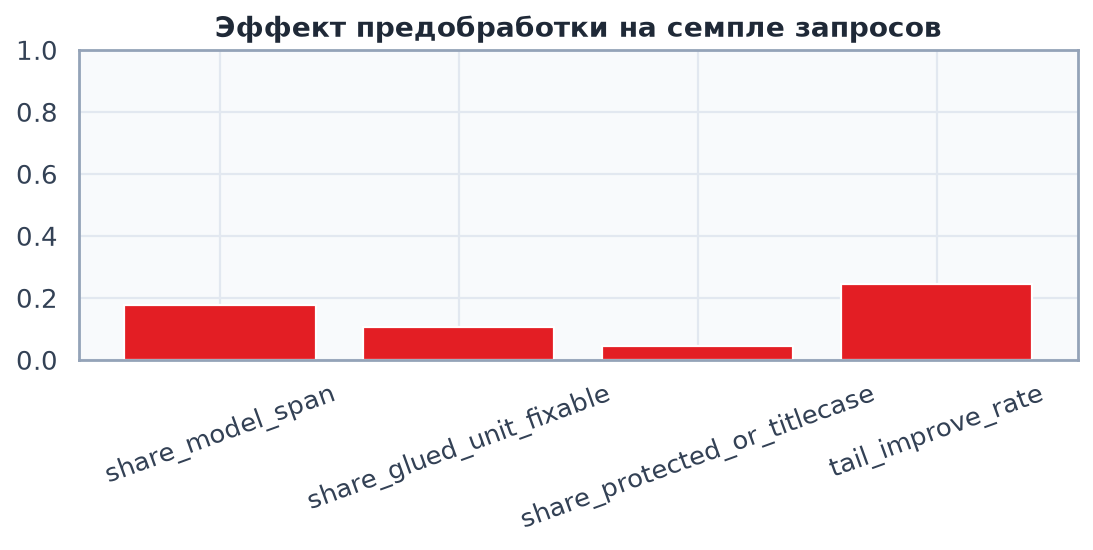
\includegraphics[width=0.94\textwidth,height=3.7cm,keepaspectratio]{02_preprocess_effect.png}
\column{0.47\textwidth}
\graynote{КАК МЕРИЛИ}{Взяли 12 000 уникальных запросов и прогнали через пайплайн дважды: со словарём моделей и без него.}
\vspace{3pt}\par
{\fontsize{7.2}{9.4}\selectfont
\numdot{1}\ 18\% запросов получают спан модели — примерно каждый пятый.\par\vspace{2pt}
\numdot{2}\ 11\% содержат склейку вида «128гб», которую чинит расклейка.\par\vspace{2pt}
\numdot{3}\ 24\% пустых хвостов после бренда получают тег модели после подсказок.\par\vspace{2pt}
\numdot{4}\ Защита брендов срабатывает у 4{,}5\% — редко, но спасает «Красный Октябрь» от превращения в цвет.}
\end{columns}
\slidefoot
\end{frame}

\begin{frame}[t]
\slidehead{тег model · проблема}{Хвост после бренда теряется}
\begin{columns}[T]
\column{0.44\textwidth}
\vspace{2pt}\centering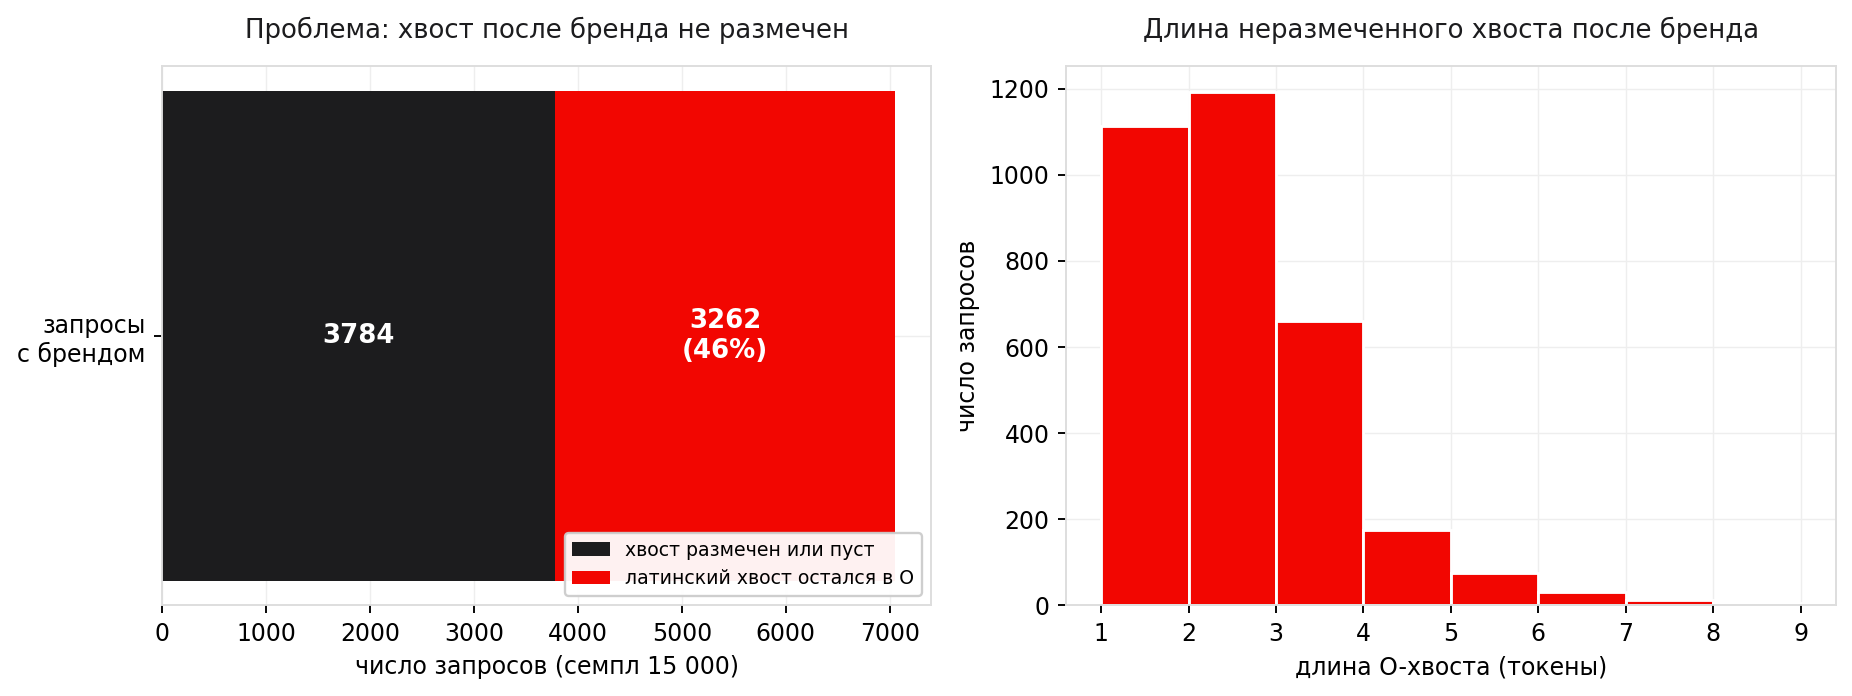
\includegraphics[width=0.96\textwidth,height=5.9cm,keepaspectratio]{model_tag/01_missing_model_problem.png}
\column{0.53\textwidth}
\pinknote{ПРОБЛЕМА}{После бренда часто идёт название линейки — «dyson v15», «galaxy s24». При слабой разметке эти слова остаются без тега, и CRF не может их выучить.}
\vspace{5pt}\par
{\smalltext
\numdot{1}\ Из 15 тысяч запросов бренд есть у 7046. Почти у половины (46\%) после бренда остался неразмеченный латинский хвост.\par\vspace{3pt}
\numdot{2}\ Типичная длина хвоста — два токена: «zenbook a16», «ipad air».\par\vspace{3pt}
\numdot{3}\ Это не атрибут — нет числа с единицей. Нужен отдельный тег MODEL и словарь линеек.}
\end{columns}
\slidefoot
\end{frame}

\begin{frame}[t]
\slidehead{тег model · примеры}{Как выглядят потерянные хвосты}
\graynote{ДО СЛОВАРЯ}{Серые слова — то, что разметка не смогла объяснить. Именно они и есть модели.}
\vspace{7pt}\par
\begin{columns}[T]
\column{0.48\textwidth}
{\InterSemi\fontsize{8}{10}\selectfont До: хвост без тега}\par\vspace{5pt}
{\fontsize{8.2}{14}\selectfont
\wtag{mvred}{пылесос} \ \wtag{mvdark}{dyson} \ \wplain{v15}\par\vspace{4pt}
\wtag{mvred}{телефон} \ \wtag{mvdark}{samsung} \ \wplain{galaxy} \ \wplain{s24}\par\vspace{4pt}
\wtag{mvdark}{asus} \ \wplain{zenbook} \ \wplain{a16}\par\vspace{4pt}
\wtag{mvdark}{apple} \ \wplain{ipad} \ \wplain{air}}
\column{0.5\textwidth}
{\InterSemi\fontsize{8}{10}\selectfont После: словарь линеек подключён}\par\vspace{5pt}
{\fontsize{8.2}{14}\selectfont
\wtag{mvred}{пылесос} \ \wtag{mvdark}{dyson} \ \wtag{okgreen}{v15 · МОДЕЛЬ}\par\vspace{4pt}
\wtag{mvred}{телефон} \ \wtag{mvdark}{samsung} \ \wtag{okgreen}{galaxy s24 · МОДЕЛЬ}\par\vspace{4pt}
\wtag{mvdark}{asus} \ \wtag{okgreen}{zenbook a16 · МОДЕЛЬ}\par\vspace{4pt}
\wtag{mvdark}{apple} \ \wtag{okgreen}{ipad air · МОДЕЛЬ}}
\end{columns}
\vspace{7pt}\par
\pinknote{ЧТО ИЗМЕНИЛОСЬ}{Хвост после бренда перестал быть «мусором» — теперь это полноценный факт «модель», по которому можно искать и ранжировать.}
\slidefoot
\end{frame}

\begin{frame}[t]
\slidehead{тег model · майнинг}{Майнинг словаря: пример «g pro»}
\graynote{ИДЕЯ}{Названия кликнутых карточек уже содержат модели. Находим в названии бренд — и всё, что идёт после него, считаем кандидатом в модели.}
\vspace{4pt}\par
\begin{columns}[T]
\column{0.49\textwidth}
{\InterSemi\fontsize{8}{10}\selectfont Название карточки $\to$ кандидаты}\par\vspace{3pt}
{\fontsize{6.8}{10}\selectfont
\wplain{Наушники} \wtag{mvdark}{Logitech} \wtag{okgreen}{G} \wtag{okgreen}{PRO} \wtag{okgreen}{X} \wtag{okgreen}{SE} \wplain{Black}}\par\vspace{3pt}
{\smalltext После бренда снимаем 1–4 коротких токена:}\par\vspace{2pt}
{\renewcommand{\arraystretch}{1.05}\setlength{\tabcolsep}{4pt}
\fontsize{7}{9}\selectfont
\begin{tabular}{|L{2.0cm}|C{1.9cm}|}
\hline
\theadl{Кандидат} & \thead{Раз}\\
\hline
\tcelll{g} & \tcellc{213}\\
\hline
\tcelll{\hb{g pro}} & \tcellc{\hnum{87}}\\
\hline
\tcelll{g pro x} & \tcellc{31}\\
\hline
\tcelll{g pro x se} & \tcellc{9}\\
\hline
\tcelll{g pro x se black} & \tcellc{2 — отсекли}\\
\hline
\end{tabular}}
\column{0.48\textwidth}
{\InterSemi\fontsize{8}{10}\selectfont Почему порог — 6 раз}\par\vspace{3pt}
{\smalltext
\numdot{1}\ Фраза попадает в словарь, если встретилась \textbf{минимум 6 раз}. «g pro» видели 87 раз — берём. «g pro x se black» — два раза, случайный хвост, отсекаем.\par\vspace{3pt}
\numdot{2}\ Порог 2 — словарь раздувается до 7215 фраз и тащит мусор. Порог 20 — остаётся 335 фраз, теряются редкие линейки.\par\vspace{3pt}
\numdot{3}\ Шесть — золотая середина: 1512 фраз, 22\% хвостов покрыто, словарь чист на 96{,}6\%.}
\end{columns}
\slidefoot
\end{frame}

\begin{frame}[t]
\slidehead{тег model · порог}{Выбор порога: размер словаря против покрытия}
\begin{columns}[T]
\column{0.5\textwidth}
\vspace{0pt}\centering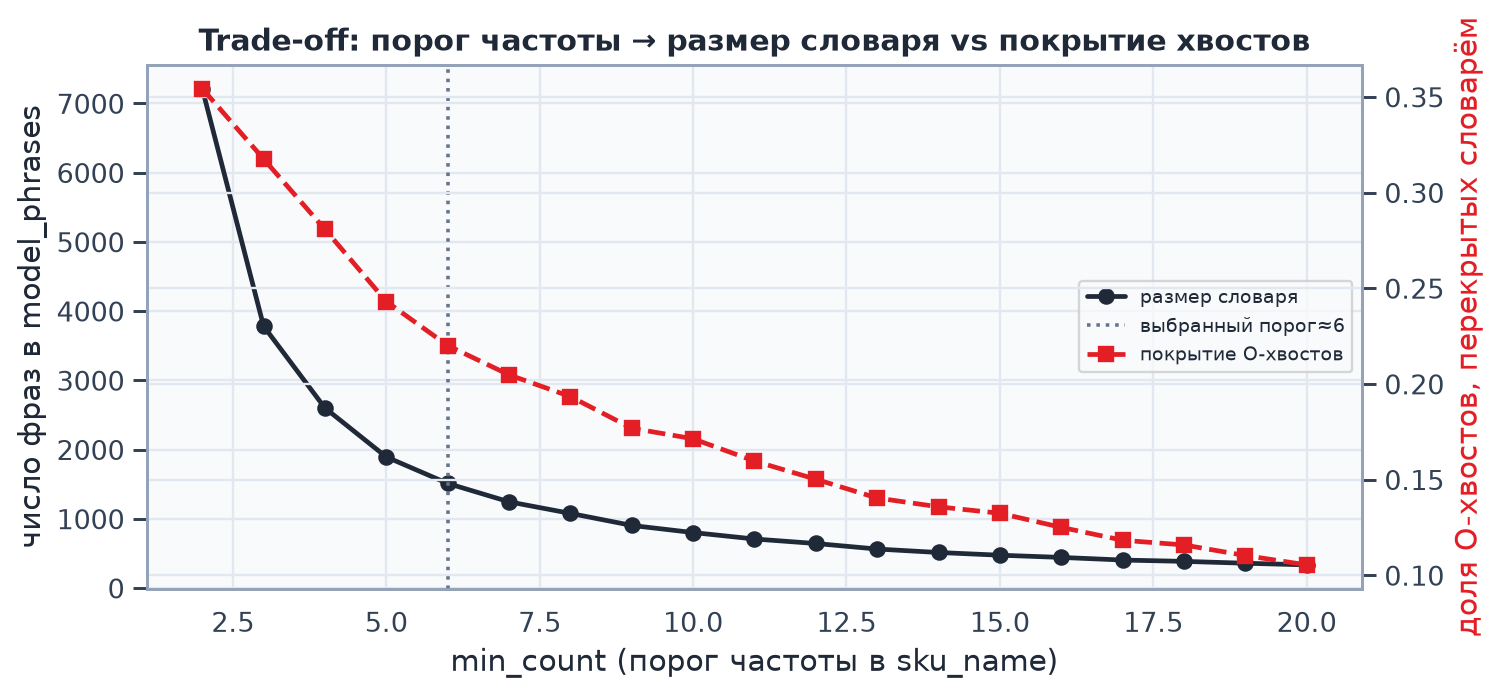
\includegraphics[width=0.94\textwidth,height=3.8cm,keepaspectratio]{model_tag/03_threshold_tradeoff.png}
\column{0.47\textwidth}
\graynote{КАК ЧИТАТЬ ГРАФИК}{Чёрная кривая — размер словаря, красная — доля хвостов, которые он покрывает. Пунктир — наш выбор.}
\vspace{3pt}\par
{\fontsize{7.2}{9.4}\selectfont
\numdot{1}\ Из 47 тысяч названий карточек намайнили 8540 сырых кандидатов: galaxy, iphone, watch, redmi и другие.\par\vspace{2.5pt}
\numdot{2}\ Кривые расходятся плавно, «локтя» нет — выбрали порог 6 как компромисс между размером и покрытием.\par\vspace{2.5pt}
\numdot{3}\ Дополнительные фильтры: голые числа не берём; фразы из одного токена — только коды вида «v15», «a305», «ps5».}
\end{columns}
\slidefoot
\end{frame}

\begin{frame}[t]
\slidehead{тег model · результат}{До и после подключения словаря}
\begin{columns}[T]
\column{0.5\textwidth}
\vspace{2pt}\centering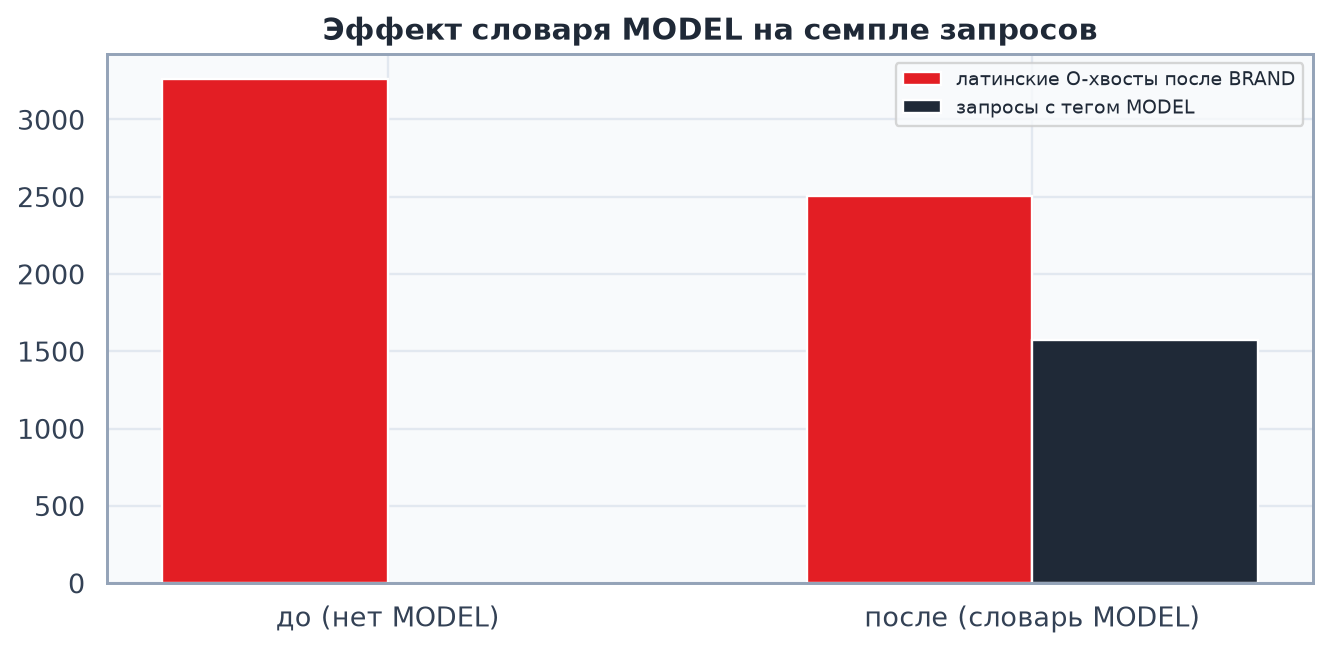
\includegraphics[width=0.98\textwidth,height=4.4cm,keepaspectratio]{model_tag/04_before_after_model_tag.png}
\column{0.47\textwidth}
\conclusion{Словарь линеек включает класс MODEL: было 0 запросов с тегом — стало 1573. Потерянных хвостов стало меньше на четверть.}
\vspace{6pt}\par
{\smalltext
\numdot{1}\ Латинские хвосты без тега: 3262 $\to$ 2502, минус 23\%.\par\vspace{4pt}
\numdot{2}\ Проверили качество словаря вручную: 96{,}6\% фраз — настоящие линейки, остальное — длинные артикулы и аксессуары, их вычистим.\par\vspace{4pt}
\numdot{3}\ Оставшиеся хвосты словарём не закрыть — это кандидаты на ручную разметку, для неё мы сделали приложение (покажем дальше).}
\end{columns}
\slidefoot
\end{frame}

\begin{frame}[t]
\slidehead{разметка · схемы}{Какие бывают схемы токен-разметки}
\graynote{КОНТЕКСТ}{Задача NER — найти спаны сущностей. Но модели классифицируют токены, поэтому спаны кодируют в токен-схему. Разные схемы — разные способы обозначить границы.}
\vspace{3pt}\par
{\renewcommand{\arraystretch}{1.12}\setlength{\tabcolsep}{5pt}
\begin{tabular}{|L{2.0cm}|C{2.3cm}|L{7.3cm}|}
\hline
\theadl{Схема} & \thead{Теги} & \theadl{Суть}\\
\hline
\tcelll{\hb{IO}} & \tcellc{I, O} & \tcelll{самое простое, но две соседние сущности сливаются}\\
\hline
\tcelll{\hb{BIO (IOB)}} & \tcellc{B, I, O} & \tcelll{B отмечает начало — границы видны; стандарт CoNLL}\\
\hline
\tcelll{\hb{IOE}} & \tcellc{I, O, E} & \tcelll{то же самое, только отмечается конец, а не начало}\\
\hline
\tcelll{\hb{BILOU}} & \tcellc{B, I, L, O, U} & \tcelll{добавляются теги конца (L) и одиночного слова (U)}\\
\hline
\tcelll{\hb{BIES}} & \tcellc{B, I, E, S, O} & \tcelll{максимум классов — сильнее дисбаланс, учить труднее}\\
\hline
\end{tabular}}
\vspace{3pt}\par
\tnote{Общая беда всех токен-схем: вложенные сущности не выразить — «адрес» нельзя разбить на город, улицу и дом одновременно.}
\slidefoot
\end{frame}

\begin{frame}[t]
\slidehead{разметка · выбор}{Храним спаны, учим на BIO}
\conclusion{Спаны — универсальный формат хранения и оценки: любой модельный ответ приводится к ним. BIO — формат обучения. Держим оба.}
\vspace{6pt}\par
\begin{columns}[T]
\column{0.5\textwidth}
{\InterSemi\fontsize{8.5}{10.5}\selectfont Почему именно BIO}\par\vspace{4pt}
{\smalltext
\numdot{1}\ Классы — полные теги (B-BRAND, I-ATTR и так далее). Буквы B, I, O лишь кодируют границы.\par\vspace{3pt}
\numdot{2}\ У 27\% запросов сущности длиннее одного токена. Схема IO склеила бы соседние сущности в одну, BIO их разделяет.\par\vspace{3pt}
\numdot{3}\ BILOU на коротких запросах даёт больше классов без выигрыша — дисбаланс растёт, качество нет.\par\vspace{3pt}
\numdot{4}\ Наши теги: BRAND, MODEL, CATEGORY, ATTR (с приставками B и I) плюс O.}
\column{0.47\textwidth}
\begin{tikzpicture}
\node[fill=cardbg, rounded corners=3pt, inner sep=8pt, text width=\dimexpr\textwidth-16pt\relax]{
{\InterSemi\fontsize{8}{10}\selectfont Пример BIO-разметки}\par\vspace{5pt}
{\fontsize{8}{12}\selectfont\color{mvdark}
ноутбук \ \biotag{mvred}{B-CATEGORY}\par\vspace{2pt}
asus \ \biotag{mvdark}{B-BRAND}\par\vspace{2pt}
zenbook \ \biotag{okgreen}{B-MODEL}\par\vspace{2pt}
16 \ \biotag{warnorange}{B-ATTR}\par\vspace{2pt}
гб \ \biotag{warnorange}{I-ATTR}}
};
\end{tikzpicture}
\end{columns}
\slidefoot
\end{frame}

\begin{frame}[t]
\slidehead{mvp · архитектура}{Гибридный каскад: MVP на тот день}
\pinknote{КАК УСТРОЕНО}{К концу дня 03 каскад выглядел так. Каждый слой закрывает слабость предыдущего: правила мгновенные, CRF понимает морфологию, дальше три классификатора — бренд, категория и тип атрибута. На выходе факты за десятки миллисекунд.}
\vspace{5pt}\par
\begin{center}
\begin{tikzpicture}[node distance=0pt]
  \node (a) {\pipestepn{mvred}{white}{ЗАПРОС\\\fontsize{5}{6}\selectfont «ноутбук asus 16 гб»}};
  \node[right=1pt of a] (c1) {\chevron};
  \node[right=1pt of c1] (b) {\pipestepn{cardbg}{mvdark}{ПРАВИЛА\\\fontsize{5}{6}\selectfont словари, regex}};
  \node[right=1pt of b] (c2) {\chevron};
  \node[right=1pt of c2] (d) {\pipestepn{cardbg}{mvdark}{CRF\\\fontsize{5}{6}\selectfont разметка токенов}};
  \node[right=1pt of d] (c3) {\chevron};
  \node[right=1pt of c3] (e) {\pipestepn{cardbg}{mvdark}{БРЕНД\\\fontsize{5}{6}\selectfont классификатор}};
  \node[right=1pt of e] (c4) {\chevron};
  \node[right=1pt of c4] (f) {\pipestepn{cardbg}{mvdark}{КАТЕГОРИЯ\\\fontsize{5}{6}\selectfont классификатор}};
  \node[right=1pt of f] (c5) {\chevron};
  \node[right=1pt of c5] (g) {\pipestepn{mvdark}{white}{АТРИБУТЫ\\\fontsize{5}{6}\selectfont классификатор}};
\end{tikzpicture}
\end{center}
\vspace{5pt}\par
\begin{center}
\begin{tikzpicture}
  \node[fill=pinkband, rounded corners=3pt, inner xsep=10pt, inner ysep=6pt,
        text width=\dimexpr\textwidth-40pt\relax, align=left] {%
    {\color{mvred}\InterBold\fontsize{8}{10}\selectfont ПЕТЛЯ КАЧЕСТВА}\hspace{7pt}%
    {\color{mvdark}\fontsize{8}{11}\selectfont неуверенные ответы и ошибки уходят в ручную разметку, на ней дообучаем CRF и пополняем словари}};
\end{tikzpicture}
\end{center}
\slidefoot
\end{frame}

\begin{frame}[t]
\slidehead{продакшен · путь запроса}{Путь запроса от строки до выдачи}
\graynote{ЗАЧЕМ}{Извлечь факты — только середина пути: дальше нормализация, каталог и ранжирование.}
\vspace{5pt}\par
\begin{center}
\begin{tikzpicture}[node distance=0pt]
  \node (p1) {\pipestepq{cardbg}{mvdark}{Запрос}};
  \node[right=1pt of p1] (a1) {\chevron};
  \node[right=1pt of a1] (p2) {\pipestepq{cardbg}{mvdark}{Пред-\\обработка}};
  \node[right=1pt of p2] (a2) {\chevron};
  \node[right=1pt of a2] (p3) {\pipestepq{mvred}{white}{Извлечение\\фактов}};
  \node[right=1pt of p3] (a3) {\chevron};
  \node[right=1pt of a3] (p4) {\pipestepq{cardbg}{mvdark}{Нормали-\\зация}};
  \node[right=1pt of p4] (a4) {\chevron};
  \node[right=1pt of a4] (p5) {\pipestepq{cardbg}{mvdark}{Каталог}};
  \node[right=1pt of p5] (a5) {\chevron};
  \node[right=1pt of a5] (p6) {\pipestepq{cardbg}{mvdark}{Ранжиро-\\вание}};
\end{tikzpicture}
\end{center}
\vspace{5pt}\par
{\renewcommand{\arraystretch}{1.1}\setlength{\tabcolsep}{7pt}
\begin{center}
\begin{tabular}{|L{3.2cm}|L{8.4cm}|}
\hline
\theadl{Шаг} & \theadl{Пример}\\
\hline
\tcelll{\hb{Нормализация}} & \tcelll{«16гб», «16 gb», «16 ГБ» — всё превращается в одно значение: 16 ГБ}\\
\hline
\tcelll{\hb{Каталог}} & \tcelll{категория «ноутбук» находит узел «Ноутбуки и планшеты»}\\
\hline
\tcelll{\hb{Ранжирование}} & \tcelll{карточки с брендом asus и памятью 16 ГБ идут наверх}\\
\hline
\end{tabular}
\end{center}}
\vspace{-2pt}
\slidefoot
\end{frame}

\begin{frame}[t]
\slidehead{mvp · классификатор бренда}{Silver для бренда: 67 классов, не только бренды}
\pinknote{КЛЮЧЕВАЯ ИДЕЯ}{Классификатор — запасной слой, когда словарь не нашёл бренд: на «холодильник» нельзя тыкать в частый клик-бренд. Поэтому в классы добавили NO\_BRAND и UNKNOWN.}
\vspace{2pt}\par
\begin{columns}[T]
\column{0.46\textwidth}
\centering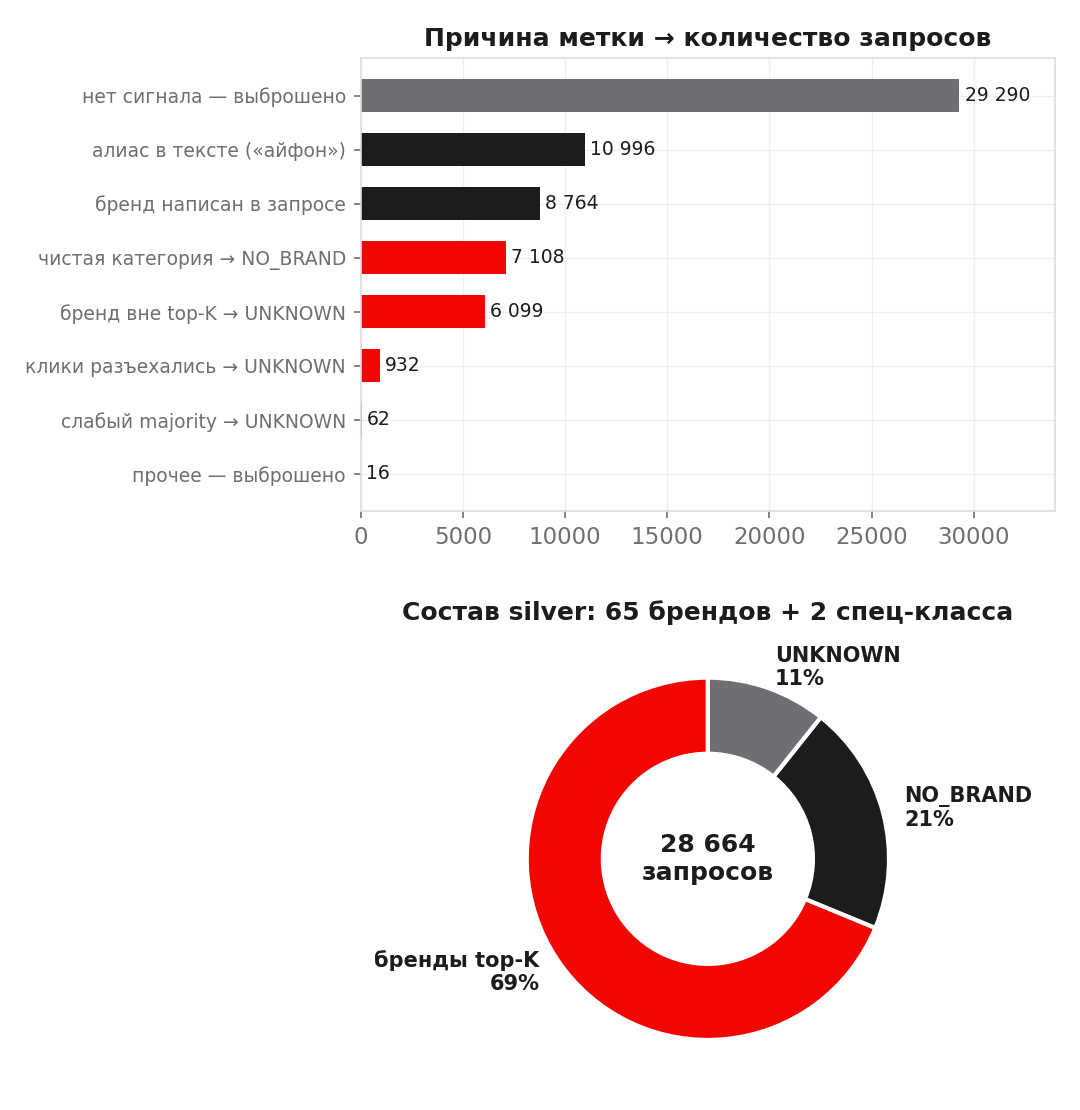
\includegraphics[width=0.95\textwidth,height=3.9cm,keepaspectratio]{brand_clf/mv_02_silver_composition.png}
\column{0.51\textwidth}
{\fontsize{7}{9}\selectfont
\numdot{1}\ Из 63 тысяч агрегированных запросов в silver попали 28 664: у остальных нет надёжного сигнала — их честно выбросили.\par\vspace{1.5pt}
\numdot{2}\ Уверенность метки — из кликов: клик выше в выдаче весит больше, майор-бренд должен набрать не меньше 55\% веса.\par\vspace{1.5pt}
\numdot{3}\ NO\_BRAND — запрос-категория без бренда. UNKNOWN — бренд есть, но вне топ-65 («стинол», «darina»): модель учится отказываться, а не угадывать похожий.\par\vspace{1.5pt}
\numdot{4}\ Разбиение: 22 846 на обучение, 5 710 на валидацию.}
\end{columns}
\slidefoot
\end{frame}

\begin{frame}[t]
\slidehead{mvp · классификатор бренда}{Четыре модели: что и как обучали}
\graynote{ПОСТАНОВКА}{Мультикласс запрос $\to$ бренд на silver. Все четыре — линейные модели на TF-IDF: отвечают за миллисекунды, критично для SLA. Разница — в признаках и балансировке.}
\vspace{3pt}\par
{\renewcommand{\arraystretch}{0.95}\setlength{\tabcolsep}{4pt}
\fontsize{6.6}{8.2}\selectfont
\begin{tabular}{|L{2.6cm}|L{4.2cm}|L{4.2cm}|}
\hline
\theadl{Модель} & \theadl{Признаки} & \theadl{Особенность}\\
\hline
\tcelll{\hb{LogReg слова+симв.}} & \tcelll{слова 1–2 + символьные n-граммы 2–4} & \tcelll{выбрана в прод: меньше всего ложных брендов}\\
\hline
\tcelll{SGD символьная} & \tcelll{символьные n-граммы} & \tcelll{лучший macro-F1, но чаще врёт на категориях}\\
\hline
\tcelll{LogReg символьная} & \tcelll{символьные n-граммы} & \tcelll{базовый вариант без словных признаков}\\
\hline
\tcelll{LogReg с балансом} & \tcelll{символьные n-граммы} & \tcelll{веса классов — хуже на редких брендах}\\
\hline
\end{tabular}}
\par\vspace{3pt}
{\smalltext
\numdot{1}\ Символьные кусочки по 2–4 буквы делают «айфон», «afon» и «iphone» похожими — опечатки не страшны.\par\vspace{2pt}
\numdot{2}\ Веса по уверенности клика: сомнительные метки влияют меньше. Все модели сохранены, сравнение — на одной валидации.}
\slidefoot
\end{frame}

\begin{frame}[t]
\slidehead{mvp · классификатор бренда}{Результаты: 0,95 macro-F1 и честные отказы}
\begin{columns}[T]
\column{0.46\textwidth}
\vspace{0pt}\centering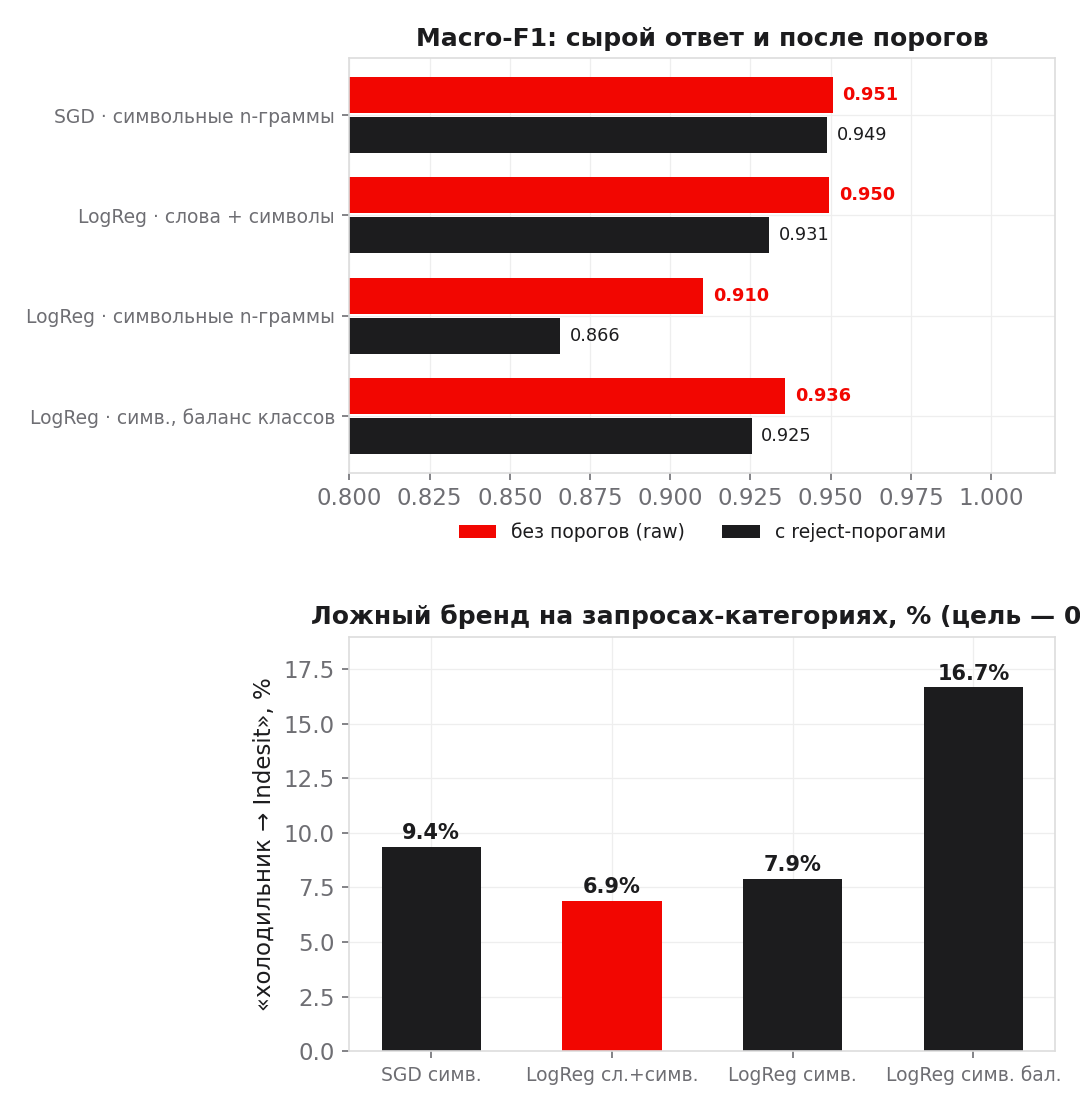
\includegraphics[width=0.94\textwidth,height=4.6cm,keepaspectratio]{brand_clf/mv_01_models_compare.png}
\column{0.51\textwidth}
\graynote{КАК ЧИТАТЬ}{Верх — macro-F1 до и после порогов отказа. Низ — доля запросов-категорий, где модель ошибочно навязала бренд (главная метрика, цель — ноль).}
\vspace{3pt}\par
{\fontsize{7.1}{9.2}\selectfont
\numdot{1}\ По macro-F1 SGD формально впереди (0{,}951 против 0{,}950), но разница — третий знак.\par\vspace{2pt}
\numdot{2}\ Решает вторая метрика: у LogReg слова+символы ложный бренд на категориях 6{,}9\% против 9{,}4\% у SGD — её и берём в прод.\par\vspace{2pt}
\numdot{3}\ F1 спец-классов: NO\_BRAND 0{,}88, UNKNOWN 0{,}86 — модель научилась говорить «бренда нет» и «не знаю».\par\vspace{2pt}
\numdot{4}\ Примеры: «айфон 15 про» даёт Apple, «холодильник» — NO\_BRAND.}
\end{columns}
\slidefoot
\end{frame}

\begin{frame}[t]
\slidehead{mvp · классификатор бренда}{Пороги отказа: лучше пусто, чем ложный бренд}
\begin{columns}[T]
\column{0.48\textwidth}
\vspace{0pt}\centering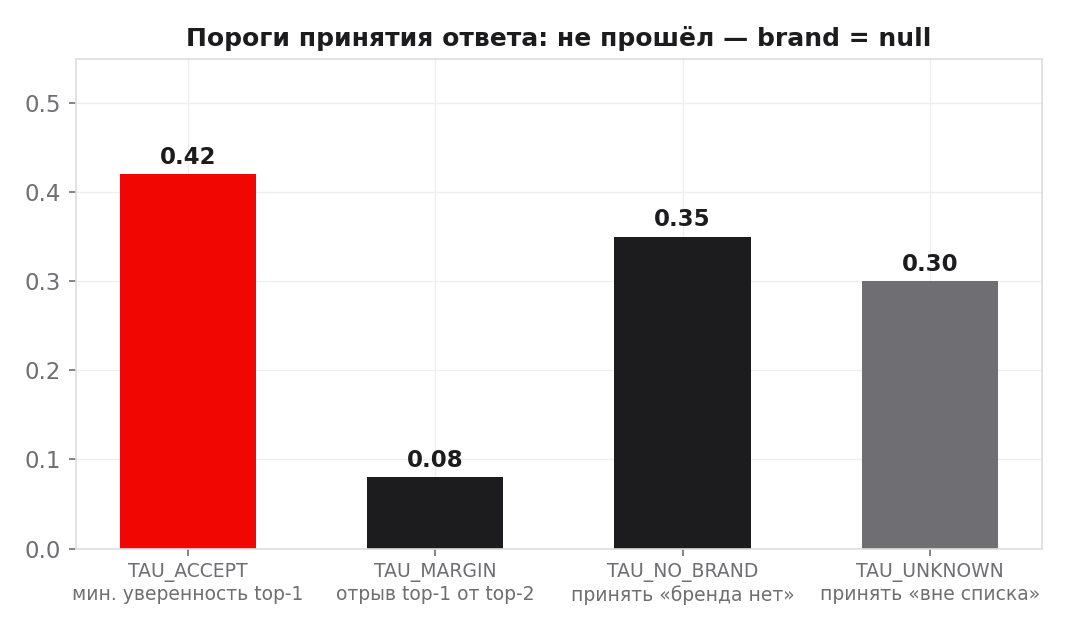
\includegraphics[width=0.94\textwidth,height=3.4cm,keepaspectratio]{brand_clf/mv_04_thresholds.png}
\par\vspace{2pt}
{\fontsize{6.8}{8.6}\selectfont\color{mvgray} Хвост по классам: PlayStation 0{,}67 (4 примера), UNKNOWN 0{,}86, NO\_BRAND 0{,}88 — редкие классы ждут золотой разметки.}
\column{0.49\textwidth}
{\fontsize{7}{9}\selectfont
{\InterSemi Когда классификатор вообще зовут:}\par\vspace{2pt}
\numdot{1}\ Словарь или алиас уже нашли бренд — не зовут.\par\vspace{2pt}
\numdot{2}\ Запрос — чистая категория — не зовут, бренд пустой.\par\vspace{2pt}
\numdot{3}\ Есть намёк на бренд (алиас, похожее на модель слово) — зовут.\par\vspace{3pt}
{\InterSemi Как принимается ответ:}\par\vspace{2pt}
\numdot{4}\ Уверенность top-1 не ниже 0{,}42 и отрыв от top-2 не меньше 0{,}08 — принимаем бренд.\par\vspace{2pt}
\numdot{5}\ Ответ NO\_BRAND или UNKNOWN выше своего порога — бренд остаётся пустым, и это правильно.\par\vspace{2pt}
\numdot{6}\ Пороги не прошли — отказ, бренд пустой. С порогами точность даже растёт: отказы съедают в основном ошибки.}
\end{columns}
\slidefoot
\end{frame}

\begin{frame}[t]
\slidehead{приложение · разметка}{Приложение разметки на C++/Qt: мастер из трёх этапов}
\graynote{КАК УСТРОЕНО}{Нативное приложение на C++ и Qt/QML. Запрос разбит на блоки по центру, фон с историей заблюрен. Этап 1: клавиши B/I/O, метка появляется над блоком, Backspace снимает и шагает назад, Enter — подтверждение этапа.}
\vspace{5pt}\par
\begin{columns}[T]
\column{0.49\textwidth}
\centering
\appshot{width=\dimexpr\textwidth-8pt\relax,height=4.6cm,keepaspectratio}{apps/cpp_label_stage1.png}\par\vspace{2pt}
{\smalltext\color{mvgray} Этап 1 — разметка B/I/O: активный блок в красной рамке, метки над блоками}
\column{0.49\textwidth}
\centering
\appshot{width=\dimexpr\textwidth-8pt\relax,height=4.6cm,keepaspectratio}{apps/cpp_label_stage2.png}\par\vspace{2pt}
{\smalltext\color{mvgray} Этап 2 — тип сущности: у каждого типа описание, когда его ставить}
\end{columns}
\slidefoot
\end{frame}

\begin{frame}[t]
\slidehead{приложение · умный поиск}{MVP умного поиска на C++/Qt}
\pinknote{КИЛЛЕР-ФИЧА}{Ранжирование каталога опирается только на извлечённые факты — бренд, категорию, модель и атрибуты, — а не на сырой текст запроса. Движок на C++ отвечает за 1–2 миллисекунды.}
\vspace{5pt}\par
\begin{columns}[T]
\column{0.49\textwidth}
\centering
\appshot{width=\dimexpr\textwidth-8pt\relax,height=4.6cm,keepaspectratio}{apps/cpp_mvp_search.png}\par\vspace{2pt}
{\smalltext\color{mvgray} Факты чипами + товары, отранжированные по фактам, с полосой релевантности}
\column{0.49\textwidth}
\centering
\appshot{width=\dimexpr\textwidth-8pt\relax,height=4.6cm,keepaspectratio}{apps/cpp_mvp_json.png}\par\vspace{2pt}
{\smalltext\color{mvgray} По клику раскрывается JSON с сущностями; таймер извлечения — в шапке}
\end{columns}
\slidefoot
\end{frame}


\daydivider{ДЕНЬ 04}{SpellFix, GLiNER и честный каскад}{Опечатки до модели, журнал экспериментов, GLiNER zero-shot/FT и joint study на gold/broken.}

\begin{frame}[t]
\slidehead{пайплайн · прод}{Гибридный каскад, который работает сейчас}
\pinknote{В ПРОДЕ}{SpellFix, правила и словари, CRF, затем классификаторы бренда, категории и атрибутов. Тот же каскад в Qt .exe, FastAPI и CLI. GLiNER измерен, в сервис пока не вшит.}
\vspace{4pt}\par
\begin{center}
\begin{tikzpicture}[node distance=0pt]
  \node (a) {\pipestepn{cardbg}{mvdark}{ЗАПРОС\\\fontsize{5}{6}\selectfont «телфон 16гь»}};
  \node[right=1pt of a] (c1) {\chevron};
  \node[right=1pt of c1] (b) {\pipestepn{mvred}{white}{SPELLFIX\\\fontsize{5}{6}\selectfont опечатки}};
  \node[right=1pt of b] (c2) {\chevron};
  \node[right=1pt of c2] (d) {\pipestepn{cardbg}{mvdark}{ПРАВИЛА\\\fontsize{5}{6}\selectfont словари}};
  \node[right=1pt of d] (c3) {\chevron};
  \node[right=1pt of c3] (e) {\pipestepn{cardbg}{mvdark}{CRF\\\fontsize{5}{6}\selectfont BIO-теги}};
\end{tikzpicture}\\[4pt]
\begin{tikzpicture}[node distance=0pt]
  \node (f) {\pipestepn{cardbg}{mvdark}{БРЕНД\\\fontsize{5}{6}\selectfont классификатор}};
  \node[right=1pt of f] (c4) {\chevron};
  \node[right=1pt of c4] (g) {\pipestepn{cardbg}{mvdark}{КАТЕГОРИЯ\\\fontsize{5}{6}\selectfont классификатор}};
  \node[right=1pt of g] (c5) {\chevron};
  \node[right=1pt of c5] (h) {\pipestepn{mvdark}{white}{АТРИБУТЫ\\\fontsize{5}{6}\selectfont классификатор}};
\end{tikzpicture}
\end{center}
\vspace{5pt}\par
{\fontsize{7.2}{9.4}\selectfont
\numdot{1}\ Каждый слой закрывает слабость предыдущего: словарь мгновенный, CRF — морфология, классификаторы — скрытый бренд, категория и тип атрибута.\par\vspace{2pt}
\numdot{2}\ Один SpellFix и при сборке silver, и в бою — модель не видит «грязный» текст только в проде.\par\vspace{2pt}
\numdot{3}\ На выходе структурированные факты, а не «чёрный ящик».}
\slidefoot
\end{frame}

\begin{frame}[t]
\slidehead{день 04 · новшества}{Что изменилось после MVP}
\pinknote{КОРОТКО}{Закрыли шум на входе, завели человекочитаемый журнал экспериментов, прогнали GLiNER как хвост и впервые измерили весь каскад на трёх типах данных.}
\vspace{10pt}\par
\begin{center}
\begin{tikzpicture}[node distance=7pt]
  \node (o1) {\iconcardsm{SpellFix}{гомоглифы, fuzzy,\\}{алиасы транслита}};
  \node[right=of o1] (o2) {\iconcardsm{CRF rebuild}{пересборка silver\\}{и рост gold microF1}};
  \node[right=of o2] (o3) {\iconcardsm{Журнал}{снимки метрик\\}{и честные кейсы}};
  \node[right=of o3] (o4) {\iconcardsm{GLiNER + joint}{один silver,\\}{метрика пайплайна}};
\end{tikzpicture}
\end{center}
\slidefoot
\end{frame}

\begin{frame}[t]
\slidehead{spellfix}{Что сделали в SpellFix}
\begin{columns}[T]
\column{0.52\textwidth}
{\InterSemi\fontsize{8.5}{10.5}\selectfont Три механики}\par\vspace{5pt}
{\renewcommand{\arraystretch}{1.3}\setlength{\tabcolsep}{5pt}
\begin{tabular}{|L{2.5cm}|L{4.0cm}|}
\hline
\theadl{Механика} & \theadl{Пример}\\
\hline
\tcelll{\hb{Fuzzy + клавиатура}} & \tcelll{«16гь» становится «16 гб», «телфон» — «телефон»}\\
\hline
\tcelll{\hb{Гомоглифы}} & \tcelll{кириллица и латиница-двойники: c/с, a/а, e/е}\\
\hline
\tcelll{\hb{Алиасы}} & \tcelll{«сони» становится «sony», «ксяоми» — «xiaomi»}\\
\hline
\end{tabular}}
\column{0.44\textwidth}
{\InterSemi\fontsize{8.5}{10.5}\selectfont Эффект на CRF}\par\vspace{5pt}
{\smalltext
SpellFix тронул \textbf{767 / 5000} silver-запросов до обучения.\par\vspace{5pt}
Gold micro-F1: \textbf{0{,}582} до правки и \textbf{0{,}594} после.\par\vspace{5pt}
Сильнее всего вырос ATTR (+0{,}07) — единицы с опечаткой больше не ломают учителя.}
\end{columns}
\vspace{6pt}\par
\conclusion{Одна функция чинит текст и при сборке обучающих данных, и в бою — без отдельного «продакшен-режима».}
\slidefoot
\end{frame}

\begin{frame}[t]
\slidehead{день 04 · журнал}{Честные кейсы и журнал экспериментов}
\begin{columns}[T]
\column{0.52\textwidth}
{\InterSemi\fontsize{8.5}{10.5}\selectfont SpellFix справляется}\par\vspace{4pt}
{\smalltext\color{mvgray}
\wplain{телфон 16 гь} \chevron\ \wplain{телефон 16 гб}\par\vspace{3pt}
\wplain{планше тxiaomi} \chevron\ \wplain{планшет xiaomi}\par\vspace{3pt}
\wplain{ноутбок asus 16гь} \chevron\ \wplain{ноутбук asus 16 гб}}
\par\vspace{7pt}
{\InterSemi\fontsize{8.5}{10.5}\selectfont Пока нет}\par\vspace{4pt}
{\smalltext\color{mvgray}
\wplain{моильник 16 гб} — слишком далёкая порча (3 буквы), вне fuzzy}
\column{0.44\textwidth}
\graynote{ЖУРНАЛ}{Папка снимков метрик CRF, brand и ATTR плюс \texttt{broken\_queries.md}. Git хранит код; сюда пишем, что поменяли и что получили.}
\vspace{6pt}\par
\pinknote{НЕ СПРЯТАЛИ}{На «sony ps5» NER ок, но классификатор категории иногда путает PlayStation с феном или смартфоном — отдельный баг, не SpellFix.}
\end{columns}
\slidefoot
\end{frame}

\begin{frame}[t]
\slidehead{gliner · zero-shot}{Что даёт модель без дообучения}
\begin{columns}[T]
\column{0.46\textwidth}
\vspace{2pt}\centering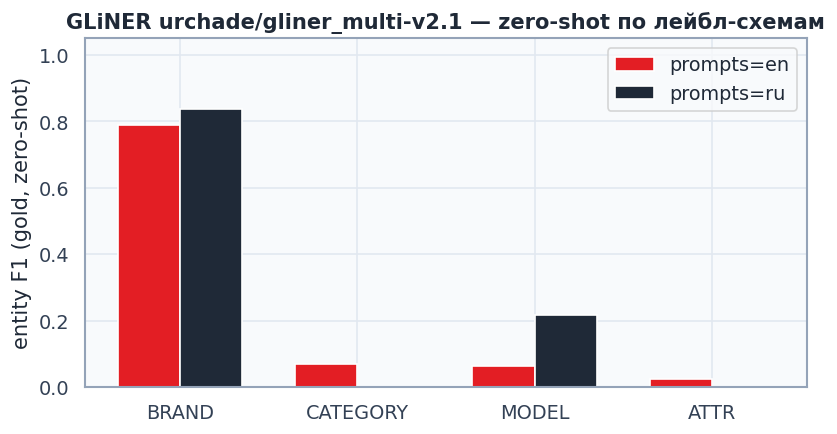
\includegraphics[width=0.95\textwidth,height=4.7cm,keepaspectratio]{01_zero_shot_f1.png}
\column{0.5\textwidth}
\graynote{МОДЕЛЬ}{\texttt{urchade/gliner\_multi-v2.1} — мультиязычный чекпоинт. Роль — гибкий хвост, не замена CRF.}
\vspace{5pt}\par
{\smalltext
\numdot{1}\ Лучшая схема промпта — английские лейблы: micro-F1 \textbf{0{,}35} на gold.\par\vspace{4pt}
\numdot{2}\ BRAND находится и без обучения (F1 $\approx$0{,}79).\par\vspace{4pt}
\numdot{3}\ CATEGORY / ATTR почти пустые — домену нужны примеры.}
\end{columns}
\slidefoot
\end{frame}

\begin{frame}[t]
\slidehead{gliner · fine-tune}{После обучения на gold + silver}
\begin{columns}[T]
\column{0.46\textwidth}
\vspace{2pt}\centering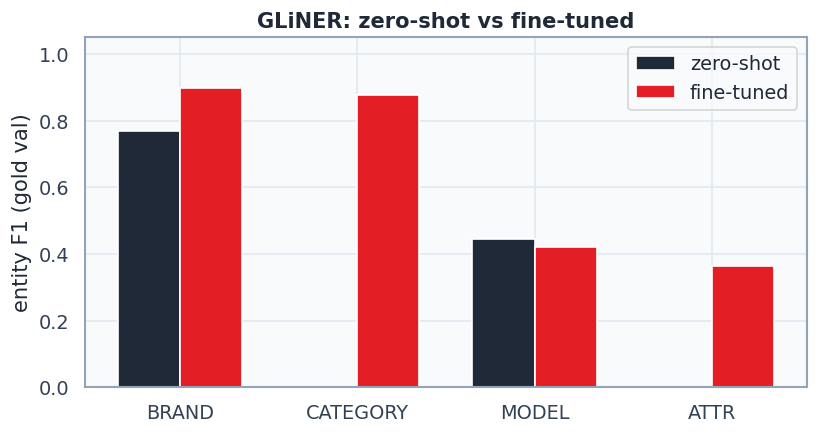
\includegraphics[width=0.95\textwidth,height=4.7cm,keepaspectratio]{02_finetune_f1.png}
\column{0.5\textwidth}
\conclusion{micro-F1 \textbf{0{,}39 $\to$ 0{,}74}: CATEGORY подтянулась с 0 до 0{,}88 — модель увидела домен.}
\vspace{5pt}\par
{\smalltext
\numdot{1}\ Порог откалиброван отдельно ($\approx$0{,}35): default 0{,}5 резал верные, но неуверенные спаны.\par\vspace{4pt}
\numdot{2}\ ATTR остаётся самым слабым (F1 $\approx$0{,}36) — мало и шумно в gold.\par\vspace{4pt}
\numdot{3}\ В прод не подключён: сначала гейт и latency-бюджет.}
\end{columns}
\slidefoot
\end{frame}

\begin{frame}[t]
\slidehead{joint study}{Один silver — честное сравнение каскада}
\pinknote{ИДЕЯ}{CRF и GLiNER на \textbf{одном} silver; gold — held-out. Стадии: rules, затем +CRF, затем +GLiNER.}
\vspace{2pt}\par
\begin{columns}[T]
\column{0.52\textwidth}
\vspace{0pt}\centering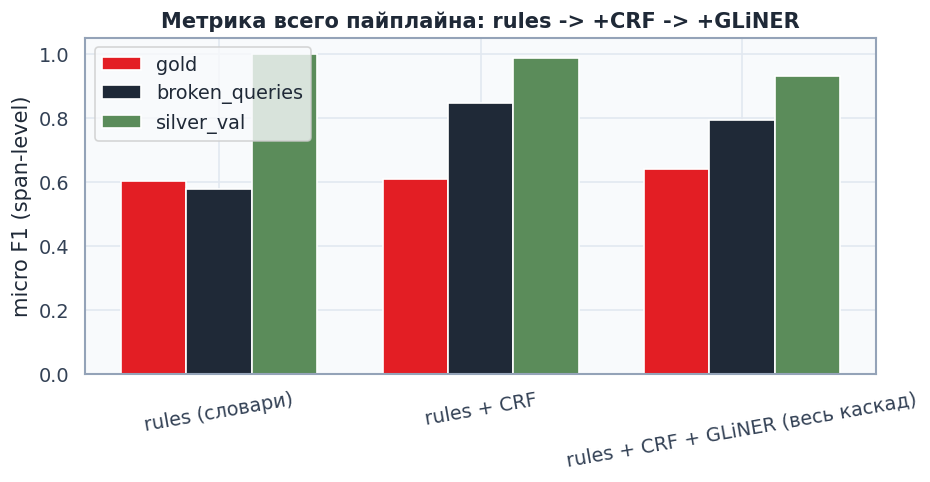
\includegraphics[width=0.95\textwidth,height=3.7cm,keepaspectratio]{02_pipeline_f1.png}
\column{0.44\textwidth}
{\fontsize{7}{9}\selectfont
\numdot{1}\ На \textbf{broken} главный прирост — CRF: \textbf{0{,}58 $\to$ 0{,}85}.\par\vspace{2pt}
\numdot{2}\ На \textbf{gold} GLiNER сверху: \textbf{0{,}61 $\to$ 0{,}64}.\par\vspace{2pt}
\numdot{3}\ На шуме «слепой» хвост \textbf{портит} precision (0{,}85$\to$0{,}80).\par\vspace{2pt}
\numdot{4}\ Silver-val $\approx$1{,}0 — самосогласие teacher, не истина.}
\end{columns}
\vspace{2pt}\par
\conclusion{GLiNER звать только когда rules+CRF ничего не нашли — не для безусловного дозаполнения.}
\slidefoot
\end{frame}

\begin{frame}[t]
\slidehead{метрики · сводка}{Честные ориентиры на одной странице}
{\renewcommand{\arraystretch}{1.28}\setlength{\tabcolsep}{5pt}
\begin{tabular}{|L{4.2cm}|C{2.4cm}|C{2.4cm}|L{3.6cm}|}
\hline
\theadl{Что} & \thead{было} & \thead{стало} & \theadl{где смотреть}\\
\hline
\tcelll{CRF gold micro-F1} & \tcellc{0{,}582} & \tcellc{\hnum{0{,}543}} & \tcelll{n=823, честный eval}\\
\hline
\tcelll{Brand clf macro-F1} & \tcellc{—} & \tcellc{\hnum{0{,}94}} & \tcelll{silver-val}\\
\hline
\tcelll{Каскад gold (rules+CRF+GL)} & \tcellc{0{,}604} & \tcellc{\hnum{0{,}640}} & \tcelll{joint study}\\
\hline
\tcelll{Каскад broken (rules+CRF)} & \tcellc{0{,}578} & \tcellc{\hnum{0{,}846}} & \tcelll{устойчивость к шуму}\\
\hline
\tcelll{GLiNER FT gold} & \tcellc{0{,}39} & \tcellc{\hnum{0{,}74}} & \tcelll{изолированный трек}\\
\hline
\end{tabular}}
\vspace{8pt}\par
\tnote{Главное правило: silver-val красивый, но завышен. Решения принимаем по gold (сейчас 823 запроса) и по broken-кейсам.}
\slidefoot
\end{frame}


\daydivider{ДЕНЬ 05}{Сервис, золотая разметка и скорость}{Подключили FastAPI и CLI, дообучили модели на ручной разметке (больше 500 товаров) и замерили, сколько миллисекунд занимает каждый слой каскада.}

% ============================================================
% ДЕНЬ 05 · FASTAPI
% ============================================================
\begin{frame}[t]
\slidehead{день 05 · fastapi}{HTTP API и CLI для того же каскада}
\pinknote{ОДИН EXTRACTOR}{Qt .exe, FastAPI и CLI ходят в одну логику: SpellFix $\to$ правила $\to$ CRF $\to$ brand/ATTR. Меняем слой один раз — проверяем тремя способами.}
\vspace{6pt}\par
\begin{columns}[T]
\column{0.48\textwidth}
{\InterSemi\fontsize{8.5}{10.5}\selectfont FastAPI (\texttt{src/service})}\par\vspace{4pt}
{\smalltext
\numdot{1}\ \texttt{POST /extract} — JSON фактов для интеграции.\par\vspace{3pt}
\numdot{2}\ \texttt{POST /extract/debug} — BIO-пайплайны для лаборатории.\par\vspace{3pt}
\numdot{3}\ \texttt{GET /health} — готовность моделей и словарей.\par\vspace{3pt}
\numdot{4}\ Веб-UI из \texttt{web/} на том же порту.}
\column{0.48\textwidth}
{\InterSemi\fontsize{8.5}{10.5}\selectfont CLI}\par\vspace{4pt}
{\smalltext
\numdot{1}\ \texttt{python -m src.cli.cli "запрос"} — smoke-тест каскада.\par\vspace{3pt}
\numdot{2}\ Режим \texttt{-i} / \texttt{--demo} для демо без UI.\par\vspace{3pt}
\numdot{3}\ Тот же \texttt{QueryEntityExtractor.from\_artifacts}.}
\end{columns}
\slidefoot
\end{frame}

% ============================================================
% ДЕНЬ 05 · GOLD + ДООБУЧЕНИЕ
% ============================================================
\begin{frame}[t]
\slidehead{день 05 · gold}{Дообучение на золотой разметке}
\conclusion{Уже размечено \textbf{более 500 товаров} под gold. GLiNER fine-tune на gold+silver: micro-F1 \textbf{0{,}39 $\to$ 0{,}74} на gold-val.}
\vspace{6pt}\par
\begin{columns}[T]
\column{0.48\textwidth}
{\InterSemi\fontsize{8.5}{10.5}\selectfont Что сделали}\par\vspace{4pt}
{\smalltext
\numdot{1}\ Gold держим как held-out: не мешаем с silver-учителем.\par\vspace{4pt}
\numdot{2}\ Fine-tune GLiNER (\texttt{urchade/gliner\_multi-v2.1}) на 154 gold + silver.\par\vspace{4pt}
\numdot{3}\ Порог откалиброван ($\approx$0{,}35) — default 0{,}5 резал верные спаны.\par\vspace{4pt}
\numdot{4}\ Разметка — в MvLabel (три аккаунта команды).}
\column{0.48\textwidth}
\vspace{2pt}\centering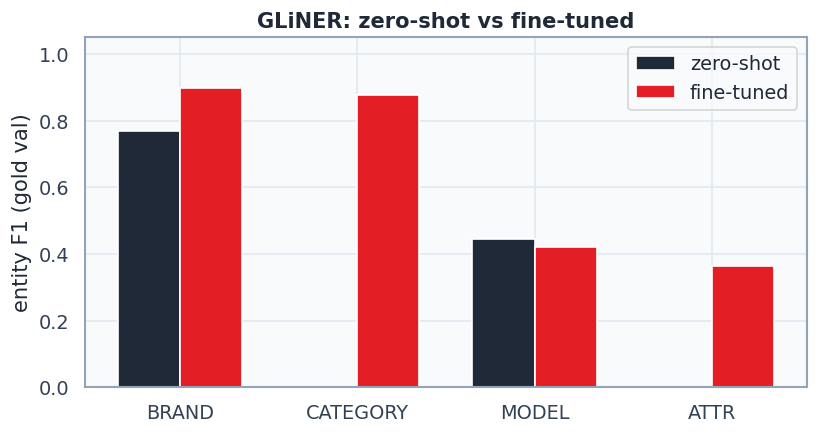
\includegraphics[width=0.95\textwidth,height=4.5cm,keepaspectratio]{02_finetune_f1.png}
\end{columns}
\slidefoot
\end{frame}

% ============================================================
% ДЕНЬ 05 · ЧЕСТНЫЙ ИНФЕРЕНС НА GOLD
% ============================================================
\begin{frame}[t]
\slidehead{день 05 · gold eval}{Честный инференс на gold: 823 запроса}
\pinknote{ЧТО СДЕЛАЛИ}{Прогнали текущий каскад на расширенном gold (\texttt{bio\_liza.jsonl}, n=823) без дообучения. Это не silver-val: здесь видно реальный потолок.}
\vspace{4pt}\par
{\renewcommand{\arraystretch}{1.2}\setlength{\tabcolsep}{5pt}
\begin{tabular}{|L{3.4cm}|C{2.0cm}|C{2.0cm}|C{2.0cm}|C{2.0cm}|}
\hline
\theadl{Слой} & \thead{micro-F1} & \thead{BRAND} & \thead{CATEGORY} & \thead{ATTR}\\
\hline
\tcelll{rules (словари)} & \tcellc{0{,}533} & \tcellc{0{,}81} & \tcellc{0{,}58} & \tcellc{0{,}28}\\
\hline
\tcelll{\hb{CRF (прод)}} & \tcellc{\hnum{0{,}543}} & \tcellc{0{,}79} & \tcellc{0{,}60} & \tcellc{0{,}29}\\
\hline
\end{tabular}}
\vspace{5pt}\par
{\fontsize{7.2}{9.4}\selectfont
\numdot{1}\ На полном gold CRF чуть выше правил (0{,}533 $\to$ 0{,}543): бренд держится, MODEL и ATTR всё ещё слабые.\par\vspace{2.5pt}
\numdot{2}\ Согласие типов атрибутов с gold: teacher 0{,}43, классификатор 0{,}54 — запасной слой ATTR полезен, но gold ещё шумный.\par\vspace{2.5pt}
\numdot{3}\ Раньше на срезе $\sim$200 запросов gold micro-F1 выглядел $\sim$0{,}59; на 823 честнее и жёстче — решения принимаем по этой цифре.}
\slidefoot
\end{frame}

% ============================================================
% ДЕНЬ 05 · LATENCY
% ============================================================
\begin{frame}[t]
\slidehead{день 05 · latency}{Скорость каскада: где укладываемся в SLA}
\pinknote{ОРИЕНТИР}{Прод-Qt / rules+CRF — десятки мс. GLiNER как хвост — $\sim$250~мс/запрос: поэтому в прод только с гейтом, не на каждый запрос.}
\vspace{6pt}\par
{\renewcommand{\arraystretch}{1.28}\setlength{\tabcolsep}{5pt}
\begin{tabular}{|L{4.2cm}|C{2.2cm}|C{2.2cm}|C{2.6cm}|}
\hline
\theadl{Стадия (gold, n=181)} & \thead{F1} & \thead{latency} & \theadl{где}\\
\hline
\tcelll{rules (словари)} & \tcellc{0{,}604} & \tcellc{\hnum{21 мс}} & \tcelll{голова}\\
\hline
\tcelll{rules + CRF} & \tcellc{0{,}609} & \tcellc{\hnum{15 мс}} & \tcelll{прод-каскад}\\
\hline
\tcelll{+ GLiNER (хвост)} & \tcellc{0{,}640} & \tcellc{249 мс} & \tcelll{эксперимент}\\
\hline
\tcelll{C++ MvSearch .exe} & \tcellc{---} & \tcellc{\hnum{1--2 мс}} & \tcelll{десктоп}\\
\hline
\end{tabular}}
\vspace{8pt}\par
{\smalltext
\numdot{1}\ На \textbf{broken\_queries} CRF даёт главный прирост (0{,}58$\to$0{,}85) при $\sim$23~мс — устойчивость к шуму без трансформера.\par\vspace{3pt}
\numdot{2}\ GLiNER zero-shot / FT: $\sim$190--210~мс на запрос — ок для офлайн-хвоста, не для SLA $<$100~мс на всём трафике.}
\slidefoot
\end{frame}

% ============================================================
% ДЕНЬ 05 · РЕПОЗИТОРИЙ
% ============================================================
\begin{frame}[t]
\slidehead{день 05 · репозиторий}{Код, релизы и презентации}
\begin{columns}[T]
\column{0.5\textwidth}
\graynote{GITHUB}{Весь пайплайн в одном репозитории:}
\vspace{6pt}\par
\begin{tikzpicture}
\node[fill=cardbg, rounded corners=4pt, inner sep=10pt, text width=\dimexpr\textwidth-20pt\relax]{%
  {\InterSemi\fontsize{10}{13}\selectfont\color{mvred}\texttt{github.com/xWooshieL/}\\[2pt]
  {\color{mvred}\texttt{mvideo-ner-search}}}\\[8pt]
  {\fontsize{8}{11}\selectfont\color{mvdark}
  Releases: \texttt{v0.4.0-final}\\[2pt]
  SmartSearch Setup 0.4.0 + Labeling 0.1.4\\[2pt]
  + итоговая презентация}
};
\end{tikzpicture}
\column{0.46\textwidth}
{\InterSemi\fontsize{8.5}{10.5}\selectfont Что внутри}\par\vspace{5pt}
{\smalltext
\numdot{1}\ C++/Qt приложения + Inno Setup.\par\vspace{4pt}
\numdot{2}\ Python: CRF, brand\_clf, SpellFix, FastAPI, CLI.\par\vspace{4pt}
\numdot{3}\ Ноутбуки: EDA, GLiNER, general\_study.\par\vspace{4pt}
\numdot{4}\ Журнал экспериментов со снимками метрик и broken-кейсами.}
\end{columns}
\slidefoot
\end{frame}


% ============================================================
% ФИНАЛ
% ============================================================
\begin{frame}[plain]
\begin{tikzpicture}[remember picture, overlay]
  \fill[mvred] (current page.south west) rectangle (current page.north east);
  \node[anchor=east, inner sep=0pt] at ([xshift=0.32\paperwidth]current page.east)
    {
\includegraphics[height=1.06\paperheight]{kurs1_image1.png}};
  \node[anchor=west, align=left] at ([xshift=0.9cm, yshift=2.35cm]current page.west)
    {\color{white}\InterBold\fontsize{23}{27}\selectfont Спасибо!};
  \node[anchor=west, align=left, text width=0.50\paperwidth] at ([xshift=0.9cm, yshift=1.35cm]current page.west)
    {\color{white}\fontsize{9.5}{12.5}\selectfont Вопросы по пайплайну, SpellFix, GLiNER и метрикам — welcome.};
  \node[anchor=west, align=left, text width=0.50\paperwidth] at ([xshift=0.9cm, yshift=-0.55cm]current page.west)
    {\color{white}\fontsize{8.5}{12}\selectfont
     {\InterSemi Команда:}\\[6pt]
     Новицкий Никита · @n.novitskiy\\[2pt]
     Борисов Никита · @n.borisov\\[2pt]
     Засухина Елизавета · @e.zasukhina\\[2pt]
     Олейников Александр · @a.oleynikov};
  \node[anchor=south west] at ([xshift=0.9cm, yshift=0.4cm]current page.south west)
    {\color{white}\fontsize{8}{10}\selectfont Презентация свёрстана в \TeX\ / \LaTeX\ · Итоги · Буткемп М.Видео};
\end{tikzpicture}
\end{frame}

\end{document}
